% Options for packages loaded elsewhere
% Options for packages loaded elsewhere
\PassOptionsToPackage{unicode}{hyperref}
\PassOptionsToPackage{hyphens}{url}
\PassOptionsToPackage{dvipsnames,svgnames,x11names}{xcolor}
%
\documentclass[
  12pt,
  letterpaper,
  DIV=11,
  numbers=noendperiod]{scrartcl}
\usepackage{xcolor}
\usepackage{amsmath,amssymb}
\setcounter{secnumdepth}{-\maxdimen} % remove section numbering
\usepackage{iftex}
\ifPDFTeX
  \usepackage[T1]{fontenc}
  \usepackage[utf8]{inputenc}
  \usepackage{textcomp} % provide euro and other symbols
\else % if luatex or xetex
  \usepackage{unicode-math} % this also loads fontspec
  \defaultfontfeatures{Scale=MatchLowercase}
  \defaultfontfeatures[\rmfamily]{Ligatures=TeX,Scale=1}
\fi
\usepackage{lmodern}
\ifPDFTeX\else
  % xetex/luatex font selection
\fi
% Use upquote if available, for straight quotes in verbatim environments
\IfFileExists{upquote.sty}{\usepackage{upquote}}{}
\IfFileExists{microtype.sty}{% use microtype if available
  \usepackage[]{microtype}
  \UseMicrotypeSet[protrusion]{basicmath} % disable protrusion for tt fonts
}{}
\makeatletter
\@ifundefined{KOMAClassName}{% if non-KOMA class
  \IfFileExists{parskip.sty}{%
    \usepackage{parskip}
  }{% else
    \setlength{\parindent}{0pt}
    \setlength{\parskip}{6pt plus 2pt minus 1pt}}
}{% if KOMA class
  \KOMAoptions{parskip=half}}
\makeatother
% Make \paragraph and \subparagraph free-standing
\makeatletter
\ifx\paragraph\undefined\else
  \let\oldparagraph\paragraph
  \renewcommand{\paragraph}{
    \@ifstar
      \xxxParagraphStar
      \xxxParagraphNoStar
  }
  \newcommand{\xxxParagraphStar}[1]{\oldparagraph*{#1}\mbox{}}
  \newcommand{\xxxParagraphNoStar}[1]{\oldparagraph{#1}\mbox{}}
\fi
\ifx\subparagraph\undefined\else
  \let\oldsubparagraph\subparagraph
  \renewcommand{\subparagraph}{
    \@ifstar
      \xxxSubParagraphStar
      \xxxSubParagraphNoStar
  }
  \newcommand{\xxxSubParagraphStar}[1]{\oldsubparagraph*{#1}\mbox{}}
  \newcommand{\xxxSubParagraphNoStar}[1]{\oldsubparagraph{#1}\mbox{}}
\fi
\makeatother


\usepackage{longtable,booktabs,array}
\newcounter{none} % for unnumbered tables
\usepackage{calc} % for calculating minipage widths
% Correct order of tables after \paragraph or \subparagraph
\usepackage{etoolbox}
\makeatletter
\patchcmd\longtable{\par}{\if@noskipsec\mbox{}\fi\par}{}{}
\makeatother
% Allow footnotes in longtable head/foot
\IfFileExists{footnotehyper.sty}{\usepackage{footnotehyper}}{\usepackage{footnote}}
\makesavenoteenv{longtable}
\usepackage{graphicx}
\makeatletter
\newsavebox\pandoc@box
\newcommand*\pandocbounded[1]{% scales image to fit in text height/width
  \sbox\pandoc@box{#1}%
  \Gscale@div\@tempa{\textheight}{\dimexpr\ht\pandoc@box+\dp\pandoc@box\relax}%
  \Gscale@div\@tempb{\linewidth}{\wd\pandoc@box}%
  \ifdim\@tempb\p@<\@tempa\p@\let\@tempa\@tempb\fi% select the smaller of both
  \ifdim\@tempa\p@<\p@\scalebox{\@tempa}{\usebox\pandoc@box}%
  \else\usebox{\pandoc@box}%
  \fi%
}
% Set default figure placement to htbp
\def\fps@figure{htbp}
\makeatother


% definitions for citeproc citations
\NewDocumentCommand\citeproctext{}{}
\NewDocumentCommand\citeproc{mm}{%
  \begingroup\def\citeproctext{#2}\cite{#1}\endgroup}
\makeatletter
 % allow citations to break across lines
 \let\@cite@ofmt\@firstofone
 % avoid brackets around text for \cite:
 \def\@biblabel#1{}
 \def\@cite#1#2{{#1\if@tempswa , #2\fi}}
\makeatother
\newlength{\cslhangindent}
\setlength{\cslhangindent}{1.5em}
\newlength{\csllabelwidth}
\setlength{\csllabelwidth}{3em}
\newenvironment{CSLReferences}[2] % #1 hanging-indent, #2 entry-spacing
 {\begin{list}{}{%
  \setlength{\itemindent}{0pt}
  \setlength{\leftmargin}{0pt}
  \setlength{\parsep}{0pt}
  % turn on hanging indent if param 1 is 1
  \ifodd #1
   \setlength{\leftmargin}{\cslhangindent}
   \setlength{\itemindent}{-1\cslhangindent}
  \fi
  % set entry spacing
  \setlength{\itemsep}{#2\baselineskip}}}
 {\end{list}}
\usepackage{calc}
\newcommand{\CSLBlock}[1]{\hfill\break\parbox[t]{\linewidth}{\strut\ignorespaces#1\strut}}
\newcommand{\CSLLeftMargin}[1]{\parbox[t]{\csllabelwidth}{\strut#1\strut}}
\newcommand{\CSLRightInline}[1]{\parbox[t]{\linewidth - \csllabelwidth}{\strut#1\strut}}
\newcommand{\CSLIndent}[1]{\hspace{\cslhangindent}#1}



\setlength{\emergencystretch}{3em} % prevent overfull lines

\providecommand{\tightlist}{%
  \setlength{\itemsep}{0pt}\setlength{\parskip}{0pt}}



 


\usepackage[left]{lineno}
\AtBeginDocument{\linenumbers}
\setlength\linenumbersep{10pt}
\KOMAoption{captions}{tableheading}
\makeatletter
\@ifpackageloaded{caption}{}{\usepackage{caption}}
\AtBeginDocument{%
\ifdefined\contentsname
  \renewcommand*\contentsname{Table of contents}
\else
  \newcommand\contentsname{Table of contents}
\fi
\ifdefined\listfigurename
  \renewcommand*\listfigurename{List of Figures}
\else
  \newcommand\listfigurename{List of Figures}
\fi
\ifdefined\listtablename
  \renewcommand*\listtablename{List of Tables}
\else
  \newcommand\listtablename{List of Tables}
\fi
\ifdefined\figurename
  \renewcommand*\figurename{Figure}
\else
  \newcommand\figurename{Figure}
\fi
\ifdefined\tablename
  \renewcommand*\tablename{Table}
\else
  \newcommand\tablename{Table}
\fi
}
\@ifpackageloaded{float}{}{\usepackage{float}}
\floatstyle{ruled}
\@ifundefined{c@chapter}{\newfloat{codelisting}{h}{lop}}{\newfloat{codelisting}{h}{lop}[chapter]}
\floatname{codelisting}{Listing}
\newcommand*\listoflistings{\listof{codelisting}{List of Listings}}
\makeatother
\makeatletter
\makeatother
\makeatletter
\@ifpackageloaded{caption}{}{\usepackage{caption}}
\@ifpackageloaded{subcaption}{}{\usepackage{subcaption}}
\makeatother
\usepackage{bookmark}
\IfFileExists{xurl.sty}{\usepackage{xurl}}{} % add URL line breaks if available
\urlstyle{same}
\hypersetup{
  pdftitle={Multi-source land-use emissions reveal rising airborne fraction},
  pdfauthor={J. Eduardo Vera-Valdes},
  pdfkeywords={airborne fraction, land-use and land-cover change
emissions, robust estimation, trend inference, multiple measurements},
  colorlinks=true,
  linkcolor={blue},
  filecolor={Maroon},
  citecolor={Blue},
  urlcolor={Blue},
  pdfcreator={LaTeX via pandoc}}


\title{Multi-source land-use emissions reveal rising airborne fraction}
\author{J. Eduardo Vera-Valdes}
\date{2026-05-30}
\begin{document}
\maketitle
\begin{abstract}
The airborne fraction is the share of anthropogenic carbon dioxide
emissions that remains in the atmosphere and is a key indicator of
carbon-cycle response and remaining carbon budgets. Whether this share
is rising remains debated because inference is sensitive to uncertainty
in land-use and land-cover change (LULC) emissions. Here we use an
expanded LULC-definition ensemble from Global Carbon Budget 2025 and
estimate airborne-fraction trends with a mixed-effects model with random
intercepts and slopes by LULC series. We find that airborne fraction
increased over 1959-2024, from about 0.41 to about 0.48, and that this
conclusion is robust to excluding the final year and to alternative
specifications that propagate denominator uncertainty. These results
clarify why earlier studies reported weak or inconclusive trend evidence
and strengthen evidence that a larger share of emitted carbon dioxide is
accumulating in the atmosphere.
\end{abstract}


\subsection*{Background}\label{background}
\addcontentsline{toc}{subsection}{Background}

The amount of anthropogenic carbon dioxide (\(CO_2\)) that can be
emitted while still meeting a given temperature goal, known as the
remaining carbon budget, depends critically on how efficiently the
land--ocean system continues to absorb \(CO_2\) emissions. In recent
decades, the share of anthropogenic \(CO_2\) emissions that remains in
the atmosphere, known as the airborne fraction (AF), has been estimated
to be around 0.45, but whether it has increased over time remains
contested\textsuperscript{1--9}.

In its classical form, AF is a yearly ratio of atmospheric growth to
total anthropogenic emissions, computed as the sum of fossil fuel
emissions and land-use and land-cover change emissions as

\begin{equation}\protect\phantomsection\label{eq-af-def}{
AF_t = \frac{G_t}{FF_t + LULC_t},
}\end{equation}

where \(G_t\) is the annual atmospheric \(CO_2\) growth, \(FF_t\) is
fossil fuel emissions excluding carbonation, and \(LULC_t\) is land-use
and land-cover change emissions. AF is a key carbon-cycle diagnostic,
with implications for carbon-cycle feedbacks and near-term mitigation
planning\textsuperscript{1,2,10}.

A persistent concern is that AF inference depends on the treatment of
land-use and land-cover change (LULC) emissions, which are uncertain and
model-dependent in annual carbon-budget accounting. The Global Carbon
Budget (GCB) 2025\textsuperscript{10} provides one column of LULC
emissions as the average of three bookkeeping models
(BLUE\textsuperscript{11}, OSCAR\textsuperscript{12},
LUCE\textsuperscript{13}), but a broader set of model-based LULC
alternatives can be constructed from the same source. Estimates that do
not incorporate this multi-source LULC information can be underpowered
and inference on trend direction becomes less reliable.

Here we address that issue with a statistical design that uses an
expanded ensemble of repeated LULC definitions in a mixed-effects trend
framework\textsuperscript{14,15} to obtain more reliable inference. The
main specification estimates AF trends from a panel of yearly AF values
constructed from each LULC measurement series, with random intercepts
and random slopes capturing between-series heterogeneity and inducing
within-series dependence over time. As a robustness exercise, we also
estimate a two-stage measurement-error weighted least squares (WLS)
model that propagates denominator uncertainty from repeated LULC
definitions into annual AF uncertainty\textsuperscript{16,17}.

Across specifications that incorporate the multi-source LULC
information, we find robust evidence that AF has increased over
1959-2024, and that this conclusion is not driven by the final
observation (2024), which shows a large AF value. By contrast, ordinary
least squares (OLS) specifications that do not incorporate denominator
measurement information provide weaker evidence of a positive trend and
are more sensitive to endpoint exclusion. Taken together, the results
clarify why AF trend significance has been elusive in the literature and
strengthen evidence that a growing share of emitted carbon dioxide is
accumulating in the atmosphere.

\subsection*{Data}\label{data}
\addcontentsline{toc}{subsection}{Data}

We use annual Global Carbon Budget 2025 data for 1959-2024, with
atmospheric growth \(G_t\) from NOAA/ESRL global concentration
trends\textsuperscript{18}, fossil emissions excluding carbonation
\(FF_t\) from the Global Carbon Project fossil
dataset\textsuperscript{10}, and a panel of 69 LULC measurements per
year: BLUE\textsuperscript{11}, OSCAR\textsuperscript{12},
LUCE\textsuperscript{13}, and peat-augmented\textsuperscript{19--21}
process-based land-model combinations drawn from the GCB model
ensemble\textsuperscript{22--42} (see Methods). The data are shown in
Figure~\ref{fig-data}.

Two LULC means can be constructed from the panel. First, the GCB LULC
mean, defined as the mean of the three bookkeeping models (BLUE, OSCAR,
and LUCE), corresponds to the LULC column used in the Global Carbon
Budget. Second, the all-LULC mean, defined as the cross-series mean
across all 69 LULC measurements. The literature has typically used the
GCB LULC mean in AF trend estimation, but we show that incorporating the
full set of LULC measurements increases the precision of trend estimates
and provides more robust inference on trend direction.

To account for the natural variability in the atmospheric growth
series\textsuperscript{5,7--9}, we construct a natural variability
adjusted growth series by regressing the observed growth on total
anthropogenic emissions (fossil plus LULC) and indices of variability in
the El Niño-Southern Oscillation (ENSO) and the Volcanic Aerosol Index
(VAI). The fitted values from this regression are used as the natural
variability adjusted growth series, which is shown in
Figure~\ref{fig-data} and used in the main analysis. The details of the
regression are described in Methods.

\begin{figure}

\centering{

\pandocbounded{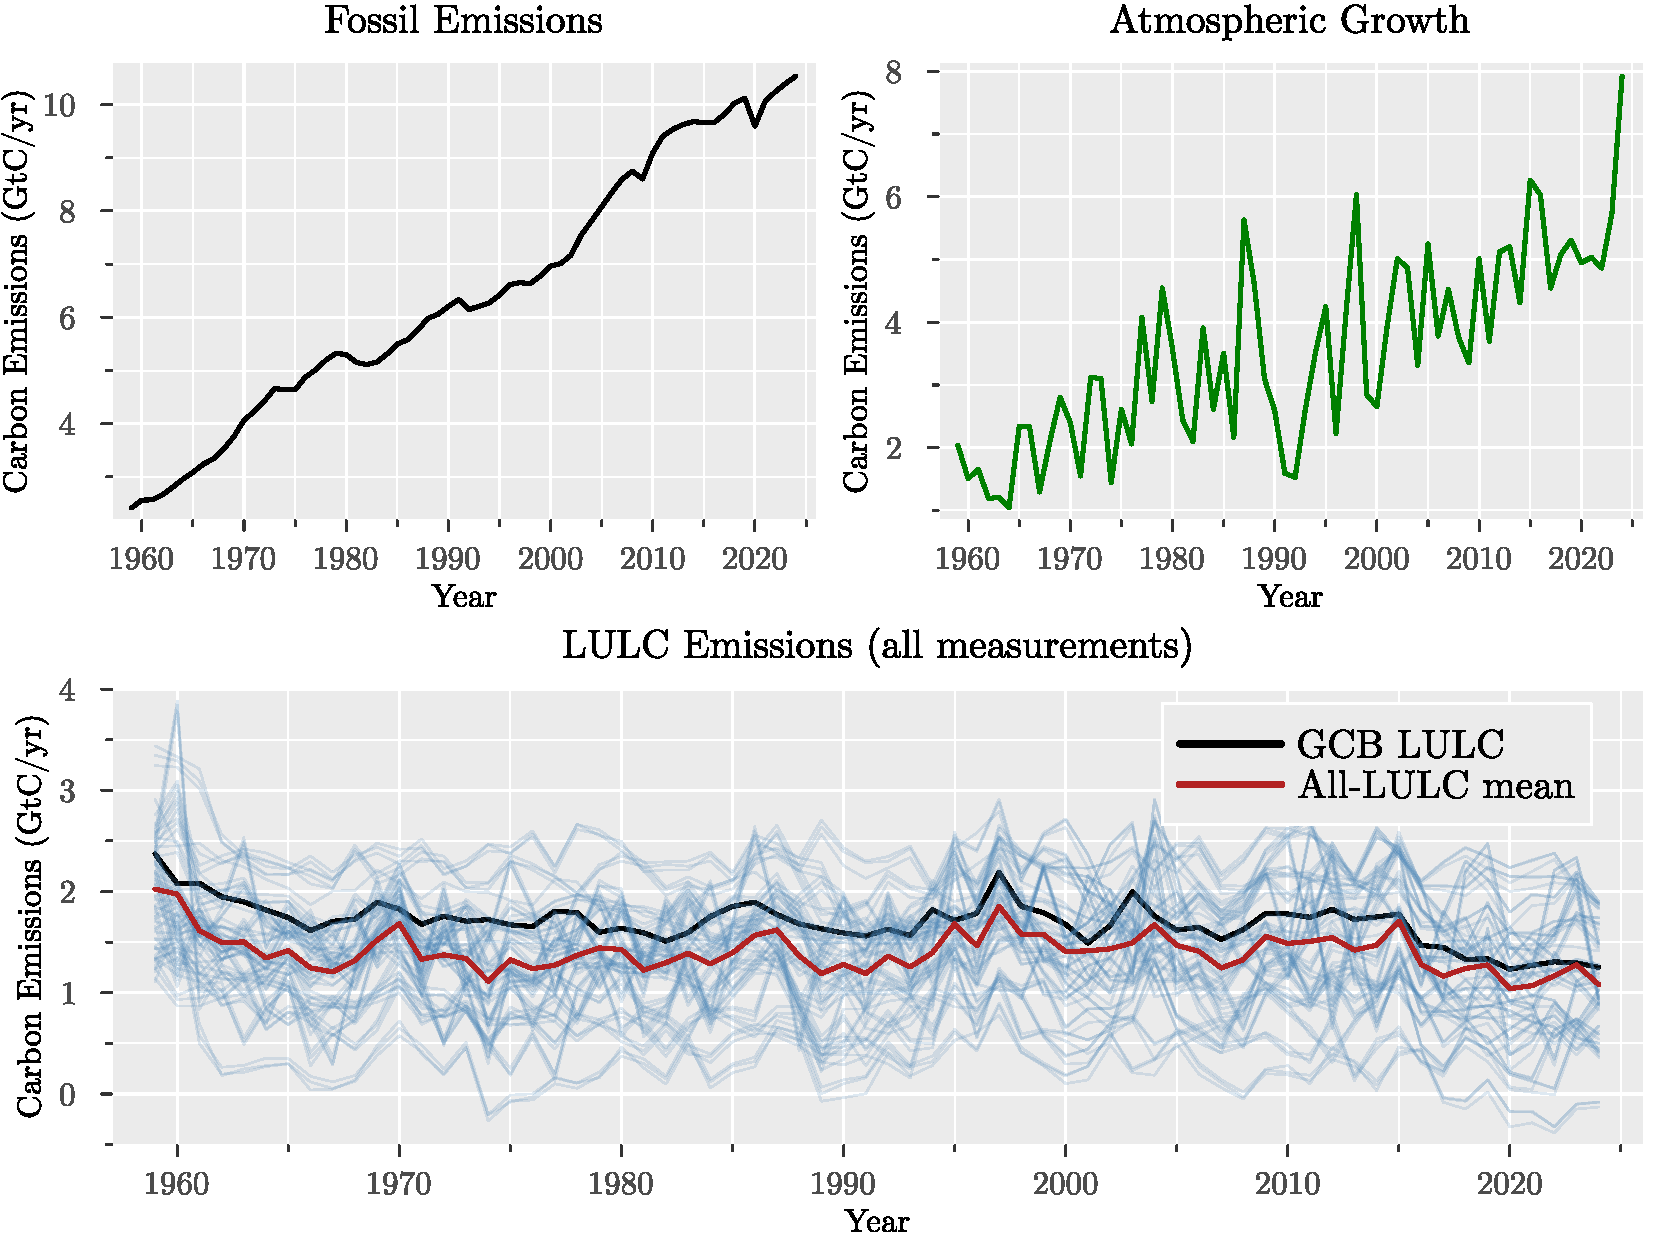
\includegraphics[keepaspectratio]{figures/af_data_all_lulc.pdf}}

}

\caption{\label{fig-data}Global Carbon Budget 2025 data for fossil
emissions, atmospheric growth, and LULC emissions (1959-2024). For
atmospheric growth, we show the observed growth and the natural
variability adjusted fit. For the LULC panel, we show all extracted and
derived LULC measurements together with the GCB LULC column and the
all-LULC cross-series mean.}

\end{figure}%

\subsection*{Identification strategy}\label{identification-strategy}
\addcontentsline{toc}{subsection}{Identification strategy}

The empirical question is whether AF has a positive linear trend. The
key design choice is how to use the full panel of repeated LULC
measurements while accounting for within-series dependence and
cross-series heterogeneity. OLS on a collapsed annual series discards
panel information and hence provides less reliable inference, as shown
in Table~\ref{tbl-trend-gcb} and Table~\ref{tbl-trend-gcb-2023}. Natural
variability in the atmospheric growth series also adds noise to AF
estimates, so we use a natural-variability-adjusted growth series in the
main analysis to obtain more precise trend estimates. Our preferred
specification is a mixed-effects model with random intercepts and random
slopes by LULC series, allowing correlation across years within each
series and capturing unobserved heterogeneity in LULC
measurements\textsuperscript{14,15} (see Methods).

For each LULC measurement series, we construct a series of AF estimates
by year (Equation~\ref{eq-af-def}), and the model estimates a common
time trend across all series while allowing for series-specific
intercepts and slopes. Formally, the model can be written as \[
AF_{t,j} = \alpha_j + \beta_j t +\varepsilon_{t,j},
\]

where

\[
\alpha_j \sim N(\mu_\alpha, \sigma_\alpha^2),\quad
\beta_j \sim N(\mu_\beta, \sigma_\beta^2),\quad
\varepsilon_{t,j} \sim N(0, \sigma_\varepsilon^2).
\]

Here \(\mu_\alpha\) and \(\mu_\beta\) are the fixed effects (overall
intercept and slope), while \(\sigma_\alpha^2\) and \(\sigma_\beta^2\)
capture the variability in intercepts and slopes across LULC measurement
series. The error term \(\varepsilon_{t,j}\) captures idiosyncratic
noise. The key parameter of interest is \(\mu_\beta\), which captures
the average trend across all LULC measurement series. Filtering growth
for natural variability and incorporating the full panel of LULC
measurements allows us to obtain more precise and robust estimates of
the AF trend.

\subsection*{Results}\label{results}
\addcontentsline{toc}{subsection}{Results}

\subsubsection*{Main estimates}\label{main-estimates}
\addcontentsline{toc}{subsubsection}{Main estimates}

The main results from estimating the mixed-effects model in the full
sample are shown in Table~\ref{tbl-mixed-effects}. The table includes
natural-variability-adjusted (\(AF^{ADJ}\)) and unadjusted
(\(AF^{RAW}\)) growth specifications, with and without AR(1) effects in
the residuals to control for potential autocorrelation (see Methods).

The slope is positive and statistically significant in all
specifications, indicating strong evidence of an increasing AF trend
across LULC measurement series. The estimated intercept is around 0.41
and the slope is around 0.0011 per year, implying an increase of about
0.07 in AF over 1959-2024. These estimates are comparable with the
approximately 0.45 AF level reported in the
literature\textsuperscript{2,3,6,7,9,43}, while identifying a positive
long-run trend when the full LULC-definition ensemble is incorporated.
Note that the mixed-effects model reduces uncertainty in the estimates
by jointly using this ensemble information, which allows us to obtain
more precise estimates and robust inference on trend direction.

\begin{longtable}[]{@{}
  >{\raggedright\arraybackslash}p{(\linewidth - 8\tabcolsep) * \real{0.2593}}
  >{\raggedleft\arraybackslash}p{(\linewidth - 8\tabcolsep) * \real{0.1852}}
  >{\raggedleft\arraybackslash}p{(\linewidth - 8\tabcolsep) * \real{0.1852}}
  >{\raggedleft\arraybackslash}p{(\linewidth - 8\tabcolsep) * \real{0.1852}}
  >{\raggedleft\arraybackslash}p{(\linewidth - 8\tabcolsep) * \real{0.1852}}@{}}
\caption{Mixed-effects model estimates for the full sample (1959-2024).
Specifications with natural variability adjusted (ADJ) and unadjusted
(RAW) growth rates are shown with and without AR(1)
effects.}\label{tbl-mixed-effects}\tabularnewline
\toprule\noalign{}
\begin{minipage}[b]{\linewidth}\raggedright
Mixed-effects model (1959-2024)
\end{minipage} & \begin{minipage}[b]{\linewidth}\raggedleft
\(AF^{ADJ}\)
\end{minipage} & \begin{minipage}[b]{\linewidth}\raggedleft
\(AF^{ADJ}\) (AR1)
\end{minipage} & \begin{minipage}[b]{\linewidth}\raggedleft
\(AF^{RAW}\)
\end{minipage} & \begin{minipage}[b]{\linewidth}\raggedleft
\(AF^{RAW}\) (AR1)
\end{minipage} \\
\midrule\noalign{}
\endfirsthead
\toprule\noalign{}
\begin{minipage}[b]{\linewidth}\raggedright
Mixed-effects model (1959-2024)
\end{minipage} & \begin{minipage}[b]{\linewidth}\raggedleft
\(AF^{ADJ}\)
\end{minipage} & \begin{minipage}[b]{\linewidth}\raggedleft
\(AF^{ADJ}\) (AR1)
\end{minipage} & \begin{minipage}[b]{\linewidth}\raggedleft
\(AF^{RAW}\)
\end{minipage} & \begin{minipage}[b]{\linewidth}\raggedleft
\(AF^{RAW}\) (AR1)
\end{minipage} \\
\midrule\noalign{}
\endhead
\bottomrule\noalign{}
\endlastfoot
Intercept & 0.407572 & 0.408555 & 0.406959 & 0.406784 \\
SE (Intercept) & 0.005324 & 0.005546 & 0.005573 & 0.005673 \\
p-value (Intercept) & 1.0E-5 & 1.0E-5 & 1.0E-5 & 1.0E-5 \\
Slope & 0.001082 & 0.00107 & 0.001103 & 0.001117 \\
SE (Slope) & 8.6E-5 & 0.0001 & 0.000102 & 0.000108 \\
p-value (Slope) & 1.0E-5 & 1.0E-5 & 1.0E-5 & 1.0E-5 \\
AR1 & & 0.177702 & & 0.063011 \\
SE (AR1) & & 0.031018 & & 0.030731 \\
p-value (AR1) & & 1.0E-5 & & 0.040326 \\
\end{longtable}

Figure~\ref{fig-mixed-effects-trend} shows the AF series for each LULC
measurement together with the overall mixed-effects trend line for the
specification using the natural-variability-adjusted growth series and
the full sample. The figure shows a clear positive trend across the
panel of AF series, with the mixed-effects model capturing this common
signal while allowing for series-specific heterogeneity. For visual
clarity, one representative AF series is highlighted, while trend lines
are estimated using the full LULC-definition ensemble.

\begin{figure}

\begin{minipage}[t]{0.50\linewidth}

\centering{

\pandocbounded{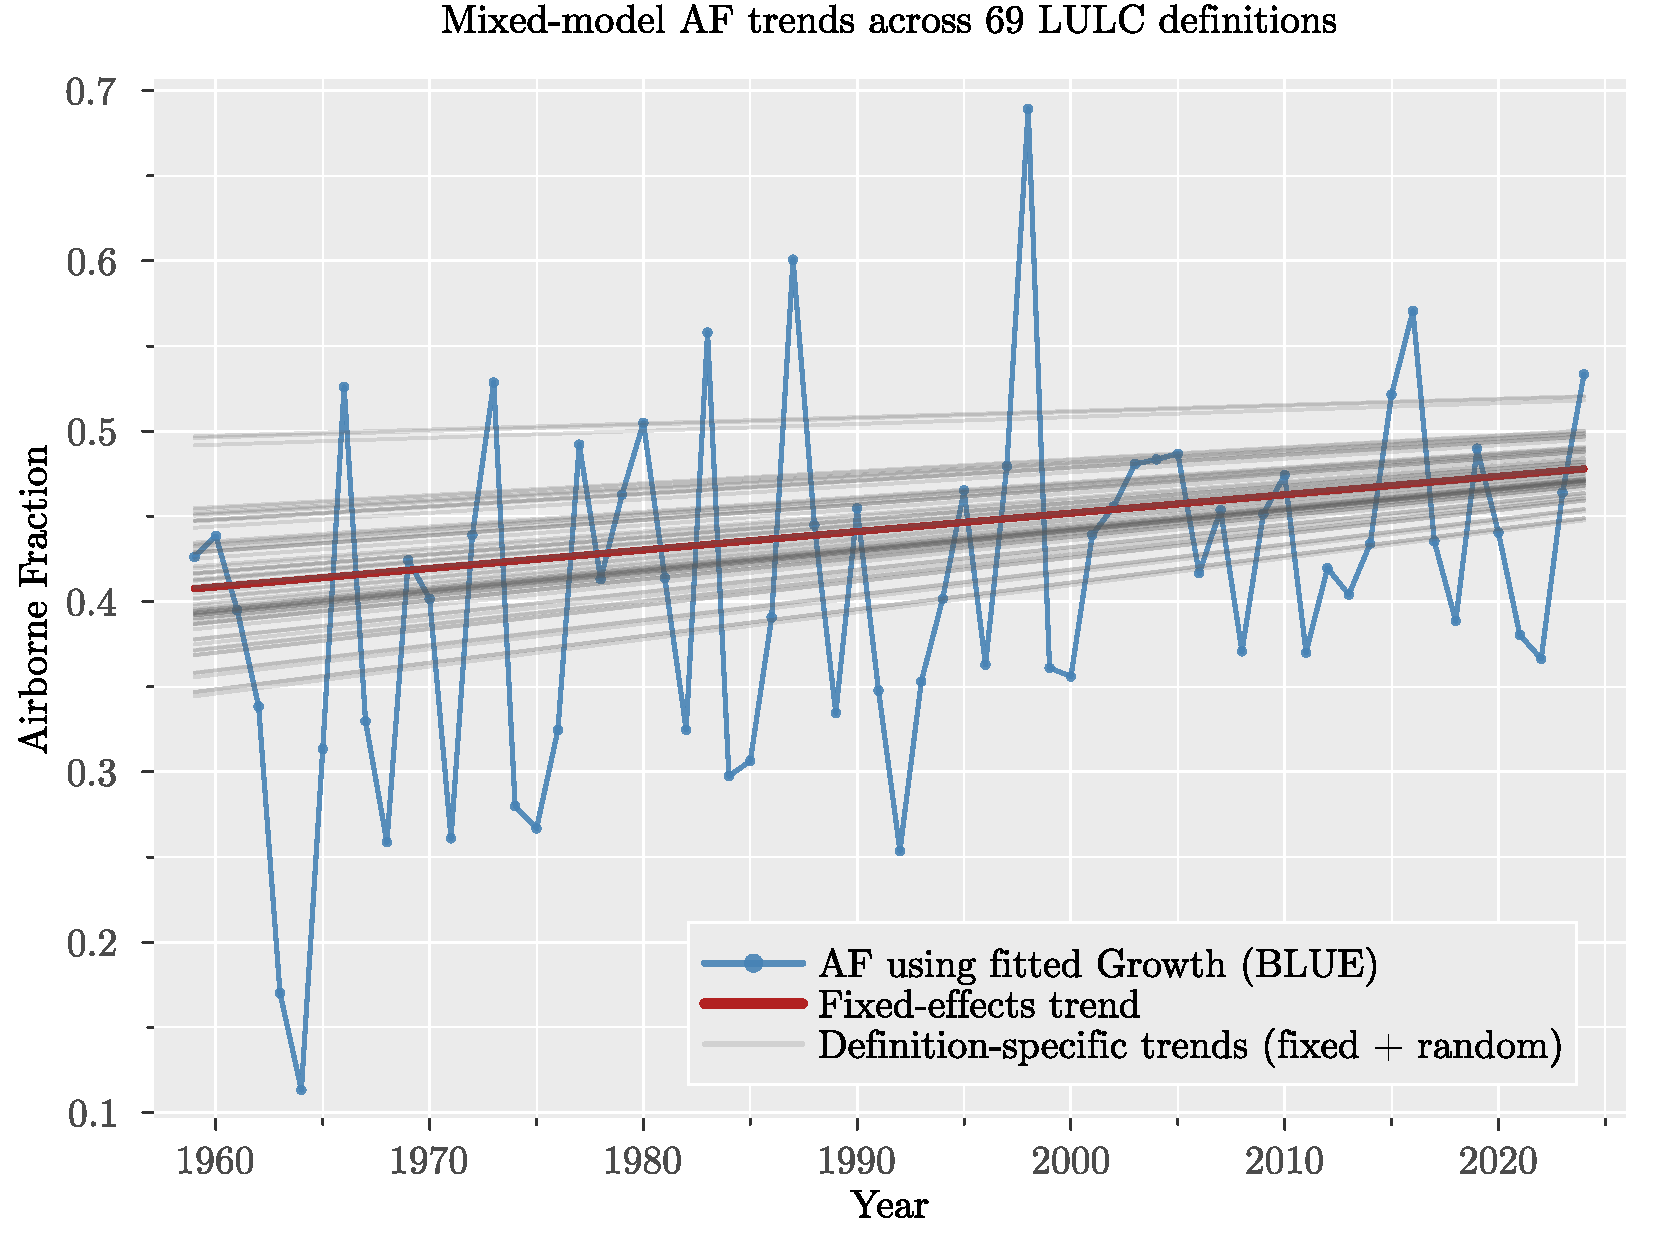
\includegraphics[keepaspectratio]{figures/AF_mixed_model_definition_trends.pdf}}

}

\subcaption{\label{fig-mixed-effects-trend}AF series with mixed-effects
model trend (natural variability adjusted, full sample, 1959-2024).}

\end{minipage}%
%
\begin{minipage}[t]{0.50\linewidth}

\centering{

\pandocbounded{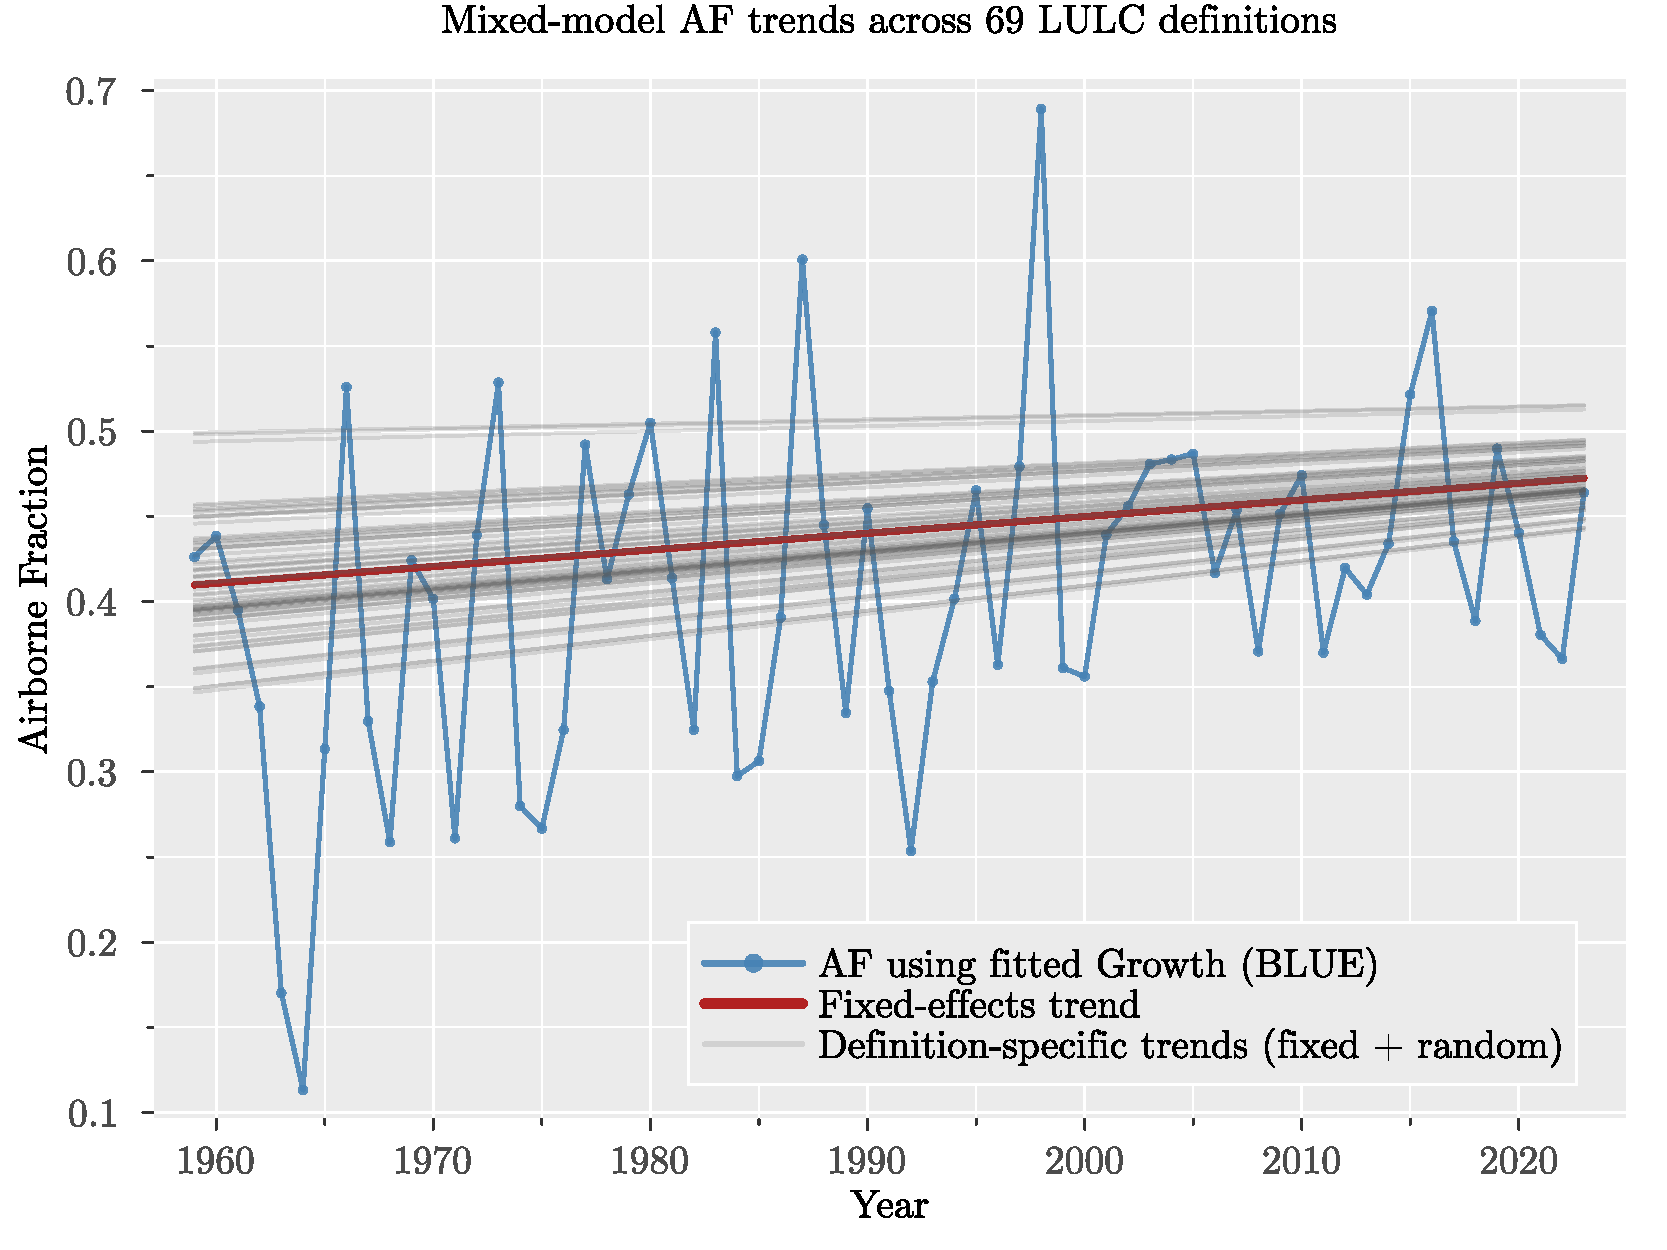
\includegraphics[keepaspectratio]{figures/AF_mixed_model_definition_trends_up_to_2023.pdf}}

}

\subcaption{\label{fig-mixed-effects-trend-2023}AF series with
mixed-effects model trend (natural variability adjusted, sample ending
in 2023).}

\end{minipage}%
\newline
\begin{minipage}[t]{0.50\linewidth}

\centering{

\pandocbounded{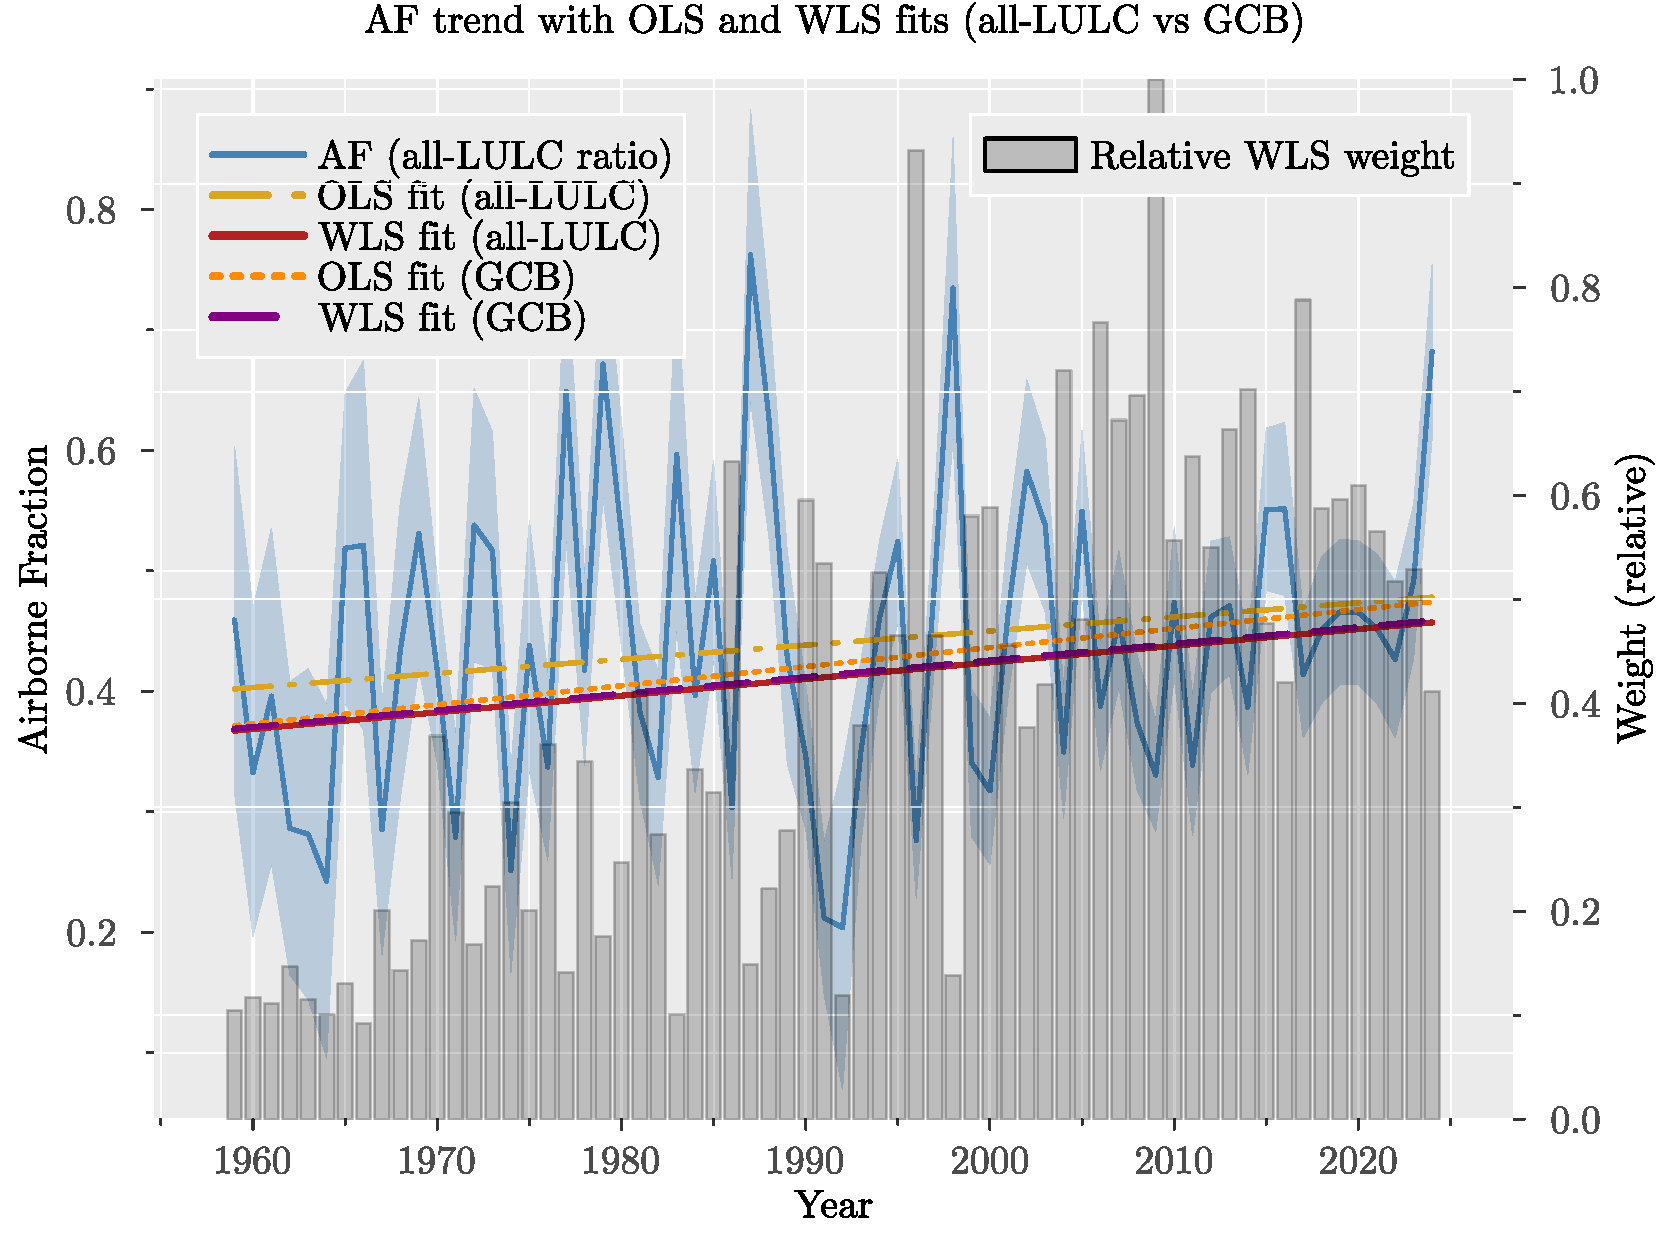
\includegraphics[keepaspectratio]{figures/AF_trends_WLS_growth.pdf}}

}

\subcaption{\label{fig-wls-trend-full}AF series with WLS trend (natural
variability adjusted, full sample, 1959-2024).}

\end{minipage}%
%
\begin{minipage}[t]{0.50\linewidth}

\centering{

\pandocbounded{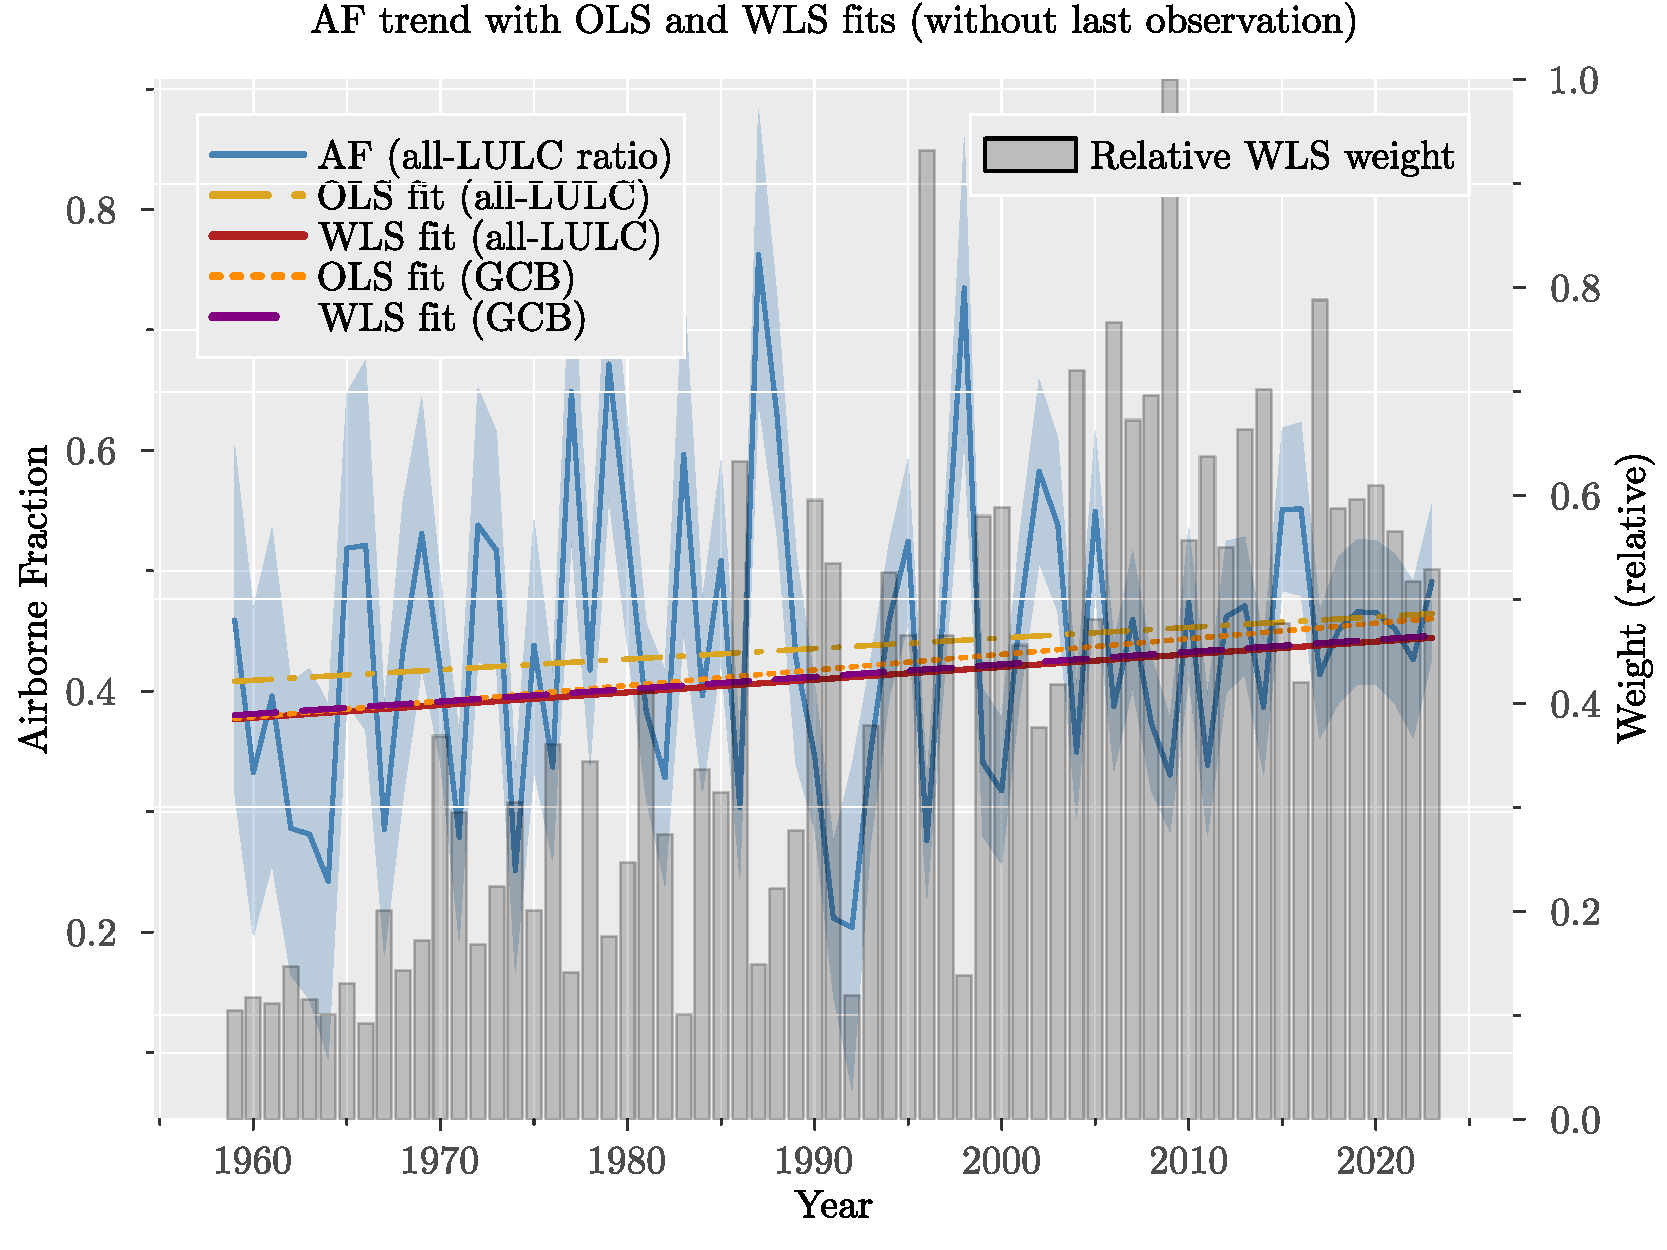
\includegraphics[keepaspectratio]{figures/AF_trends_WLS_growth_without_last_observation.pdf}}

}

\subcaption{\label{fig-wls-trend-2023}AF series with WLS trend (natural
variability adjusted, sample ending in 2023).}

\end{minipage}%

\caption{\label{fig-mixed-effects}AF series with mixed-effects and WLS
model trends across LULC measurement series.}

\end{figure}%

\subsubsection*{Endpoint and model specification
robustness}\label{endpoint-and-model-specification-robustness}
\addcontentsline{toc}{subsubsection}{Endpoint and model specification
robustness}

AF shows a large value in the final year (2024), so we re-estimate the
mixed-effects specification on the sample ending in 2023 to check
whether the result is driven by that observation. Results are shown in
Table~\ref{tbl-mixed-effects-2023} and
Figure~\ref{fig-mixed-effects-trend-2023}. The slope remains positive
and statistically significant, indicating that the increasing AF trend
is not driven by the final observation. The slope estimates are smaller,
consistent with a contribution from the 2024 large value, but the
direction and inference are unchanged.

\begin{longtable}[]{@{}
  >{\raggedright\arraybackslash}p{(\linewidth - 8\tabcolsep) * \real{0.2593}}
  >{\raggedleft\arraybackslash}p{(\linewidth - 8\tabcolsep) * \real{0.1852}}
  >{\raggedleft\arraybackslash}p{(\linewidth - 8\tabcolsep) * \real{0.1852}}
  >{\raggedleft\arraybackslash}p{(\linewidth - 8\tabcolsep) * \real{0.1852}}
  >{\raggedleft\arraybackslash}p{(\linewidth - 8\tabcolsep) * \real{0.1852}}@{}}
\caption{Mixed-effects model estimates for the sample ending in 2023
(1959-2023). Specifications with natural variability adjusted (ADJ) and
unadjusted (RAW) growth rates are shown with and without AR(1)
effects.}\label{tbl-mixed-effects-2023}\tabularnewline
\toprule\noalign{}
\begin{minipage}[b]{\linewidth}\raggedright
Mixed-effects model (1959-2023)
\end{minipage} & \begin{minipage}[b]{\linewidth}\raggedleft
\(AF^{ADJ}\)
\end{minipage} & \begin{minipage}[b]{\linewidth}\raggedleft
\(AF^{ADJ}\) (AR1)
\end{minipage} & \begin{minipage}[b]{\linewidth}\raggedleft
\(AF^{RAW}\)
\end{minipage} & \begin{minipage}[b]{\linewidth}\raggedleft
\(AF^{RAW}\) (AR1)
\end{minipage} \\
\midrule\noalign{}
\endfirsthead
\toprule\noalign{}
\begin{minipage}[b]{\linewidth}\raggedright
Mixed-effects model (1959-2023)
\end{minipage} & \begin{minipage}[b]{\linewidth}\raggedleft
\(AF^{ADJ}\)
\end{minipage} & \begin{minipage}[b]{\linewidth}\raggedleft
\(AF^{ADJ}\) (AR1)
\end{minipage} & \begin{minipage}[b]{\linewidth}\raggedleft
\(AF^{RAW}\)
\end{minipage} & \begin{minipage}[b]{\linewidth}\raggedleft
\(AF^{RAW}\) (AR1)
\end{minipage} \\
\midrule\noalign{}
\endhead
\bottomrule\noalign{}
\endlastfoot
Intercept & 0.409783 & 0.411223 & 0.41326 & 0.413403 \\
SE (Intercept) & 0.005345 & 0.005564 & 0.005586 & 0.005677 \\
p-value (Intercept) & 1.0E-5 & 1.0E-5 & 1.0E-5 & 1.0E-5 \\
Slope & 0.000978 & 0.000944 & 0.000808 & 0.000806 \\
SE (Slope) & 8.8E-5 & 0.000102 & 0.000103 & 0.000109 \\
p-value (Slope) & 1.0E-5 & 1.0E-5 & 1.0E-5 & 1.0E-5 \\
AR1 & & 0.17795 & & 0.056406 \\
SE (AR1) & & 0.031115 & & 0.029828 \\
p-value (AR1) & & 1.0E-5 & & 0.058622 \\
\end{longtable}

An additional estimation approach that explicitly incorporates
denominator measurement uncertainty is WLS estimation of the AF trend,
where the weights are constructed from the cross-measurement dispersion
of the full LULC panel. Specifically, we estimate a delta-method
uncertainty proxy for each annual AF estimate using the
cross-measurement dispersion of the full 69-series LULC panel, and use
these proxies in a WLS specification\textsuperscript{16,17,44} (see
Methods). Table~\ref{tbl-trend-WLS} reports the results using the
all-LULC mean in the denominator estimated by OLS and WLS. The first two
columns show the full sample (1959-2024) estimates, while the last two
columns show the estimates for the sample ending in 2023 to check
whether the results are driven by the large value in 2024. The WLS
estimates show a positive and statistically significant slope in both
samples, while OLS estimates show a positive but non-significant slope
in both samples. Figure~\ref{fig-wls-trend-full} and
Figure~\ref{fig-wls-trend-2023} show the WLS trend lines together with
the AF series for each LULC measurement for the full sample and the
sample ending in 2023, respectively. The WLS trend lines show a clear
positive trend across the panel of AF series.

\begin{longtable}[]{@{}
  >{\raggedright\arraybackslash}p{(\linewidth - 8\tabcolsep) * \real{0.3043}}
  >{\raggedleft\arraybackslash}p{(\linewidth - 8\tabcolsep) * \real{0.1739}}
  >{\raggedleft\arraybackslash}p{(\linewidth - 8\tabcolsep) * \real{0.1739}}
  >{\raggedleft\arraybackslash}p{(\linewidth - 8\tabcolsep) * \real{0.1739}}
  >{\raggedleft\arraybackslash}p{(\linewidth - 8\tabcolsep) * \real{0.1739}}@{}}
\caption{Trend comparison for the WLS and OLS estimates with natural
variability adjusted growth specifications. The first two columns show
the full sample (1959-2024) estimates, while the last two columns show
the estimates for the sample ending in
2023.}\label{tbl-trend-WLS}\tabularnewline
\toprule\noalign{}
\begin{minipage}[b]{\linewidth}\raggedright
OLS and WLS
\end{minipage} & \begin{minipage}[b]{\linewidth}\raggedleft
\(AF^{ADJ}\) OLS (1959-2024)
\end{minipage} & \begin{minipage}[b]{\linewidth}\raggedleft
\(AF^{ADJ}\) WLS (1959-2024)
\end{minipage} & \begin{minipage}[b]{\linewidth}\raggedleft
\(AF^{ADJ}\) OLS (1959-2023)
\end{minipage} & \begin{minipage}[b]{\linewidth}\raggedleft
\(AF^{ADJ}\) WLS (1959-2023)
\end{minipage} \\
\midrule\noalign{}
\endfirsthead
\toprule\noalign{}
\begin{minipage}[b]{\linewidth}\raggedright
OLS and WLS
\end{minipage} & \begin{minipage}[b]{\linewidth}\raggedleft
\(AF^{ADJ}\) OLS (1959-2024)
\end{minipage} & \begin{minipage}[b]{\linewidth}\raggedleft
\(AF^{ADJ}\) WLS (1959-2024)
\end{minipage} & \begin{minipage}[b]{\linewidth}\raggedleft
\(AF^{ADJ}\) OLS (1959-2023)
\end{minipage} & \begin{minipage}[b]{\linewidth}\raggedleft
\(AF^{ADJ}\) WLS (1959-2023)
\end{minipage} \\
\midrule\noalign{}
\endhead
\bottomrule\noalign{}
\endlastfoot
Intercept & 0.401938 & 0.367286 & 0.408212 & 0.376919 \\
SE (Intercept) & 0.029843 & 0.001243 & 0.029599 & 0.001211 \\
p-value (Intercept) & 1.0E-5 & 1.0E-5 & 1.0E-5 & 1.0E-5 \\
Slope & 0.001172 & 0.001382 & 0.000878 & 0.001054 \\
SE (Slope) & 0.000792 & 2.8E-5 & 0.000798 & 2.8E-5 \\
p-value (Slope) & 0.138912 & 1.0E-5 & 0.271089 & 1.0E-5 \\
\end{longtable}

Overall, the results show that incorporating multi-source LULC
information and accounting for measurement uncertainty materially
changes inference on AF trends. The mixed-effects model, which
incorporates the full LULC-definition ensemble and accounts for
within-series dependence and cross-series heterogeneity, provides robust
evidence of a positive AF trend. The WLS approach, which explicitly
incorporates denominator measurement uncertainty, also shows a positive
and statistically significant trend.

In contrast, OLS specifications that do not incorporate denominator
measurement information provide weaker and less robust evidence, with
significance that is sensitive to denominator definition and endpoint
exclusion. These results highlight the value of incorporating
multi-source LULC information in AF trend estimation in a way that
accounts for within-series dependence and cross-series heterogeneity.
OLS on a collapsed series discards this information and hence provides
less reliable inference on trend direction. Our results clarify why
earlier studies that did not incorporate multi-source LULC information
have reported weak or inconclusive evidence of an increasing AF
trend\textsuperscript{1--8}.

Additional robustness checks (in Methods), including OLS and WLS
specifications in the unadjusted growth series and considering the GCB
LULC mean instead of the all-LULC mean, show that the positive AF trend
detected by WLS is robust to these alternative specifications, while OLS
estimates that do not incorporate multi-source LULC information show
weaker evidence of a positive trend and are more sensitive to endpoint
exclusion.

\subsection*{Discussion and conclusion}\label{discussion-and-conclusion}
\addcontentsline{toc}{subsection}{Discussion and conclusion}

Using a framework that controls for natural variability in the
atmospheric growth series and incorporates a broad LULC-definition
ensemble from Global Carbon Budget 2025, we find robust evidence that AF
increased from 1959 to 2024. Methodologically, incorporating
multi-source uncertainty materially changes inference relative to plain
OLS. Endpoint tests show that this conclusion is not driven by the large
value in 2024.

Our estimates imply that AF increased from about 0.41 around 1960 to
about 0.48 by 2024, relative to long-used values around 0.45. For a
given emissions pathway, a higher AF would be associated with faster
atmospheric \(CO_2\) growth than under a constant-AF baseline,
potentially reducing the remaining carbon budget for a given temperature
target\textsuperscript{1,2,10}. Quantifying the budget impact requires
dedicated carbon-budget modelling beyond the scope of this study.

\protect\phantomsection\label{refs}
\begin{CSLReferences}{0}{0}
\bibitem[\citeproctext]{ref-Canadell2007}
\CSLLeftMargin{1. }%
\CSLRightInline{Canadell, J. G. \emph{et al.}
\href{https://doi.org/10.1073/pnas.0702737104}{Contributions to
accelerating atmospheric {CO\(_2\)} growth from economic activity,
carbon intensity, and efficiency of natural sinks}. \emph{Proceedings of
the National Academy of Sciences} \textbf{104}, 18866--18870 (2007).}

\bibitem[\citeproctext]{ref-Raupach2007}
\CSLLeftMargin{2. }%
\CSLRightInline{Raupach, M. R. \emph{et al.}
\href{https://doi.org/10.1073/pnas.0700609104}{Global and regional
drivers of accelerating {CO\(_2\)} emissions}. \emph{Proceedings of the
National Academy of Sciences} \textbf{104}, 10288--10293 (2007).}

\bibitem[\citeproctext]{ref-Knorr2009}
\CSLLeftMargin{3. }%
\CSLRightInline{Knorr, W. \href{https://doi.org/10.1029/2009GL040613}{Is
the airborne fraction of anthropogenic {CO\(_2\)} emissions increasing?}
\emph{Geophysical Research Letters} \textbf{36}, L21710 (2009).}

\bibitem[\citeproctext]{ref-Ballantyne2012}
\CSLLeftMargin{4. }%
\CSLRightInline{Ballantyne, A. P., Alden, C. B., Miller, J. B., Tans, P.
P. \& White, J. W. C.
\href{https://doi.org/10.1038/nature11299}{Increase in observed net
carbon dioxide uptake by land and oceans during the past 50 years}.
\emph{Nature} \textbf{488}, 70--72 (2012).}

\bibitem[\citeproctext]{ref-LeQuere2009}
\CSLLeftMargin{5. }%
\CSLRightInline{Le Quéré, C. \emph{et al.}
\href{https://doi.org/10.1038/ngeo689}{Trends in the sources and sinks
of carbon dioxide}. \emph{Nature Geoscience} \textbf{2}, 831--836
(2009).}

\bibitem[\citeproctext]{ref-bennedsenEvidenceTrendCO22023}
\CSLLeftMargin{6. }%
\CSLRightInline{Bennedsen, M., Hillebrand, E. \& Koopman, S. J.
\href{https://doi.org/10.1038/s41586-023-05871-6}{On the evidence of a
trend in the {CO2} airborne fraction}. \emph{Nature} \textbf{616},
E1--E3 (2023).}

\bibitem[\citeproctext]{ref-bennedsenRegressionbasedApproachCO22024}
\CSLLeftMargin{7. }%
\CSLRightInline{Bennedsen, M., Hillebrand, E. \& Koopman, S. J.
\href{https://doi.org/10.1038/s41467-024-52728-1}{A regression-based
approach to the {CO2} airborne fraction}. \emph{Nature Communications}
\textbf{15}, 8507 (2024).}

\bibitem[\citeproctext]{ref-bennettQuantificationAirborneFraction2024}
\CSLLeftMargin{8. }%
\CSLRightInline{Bennett, B. F., Salawitch, R. J., McBride, L. A., Hope,
A. P. \& Tribett, W. R.
\href{https://doi.org/10.1029/2023JG007760}{Quantification of the
{Airborne} {Fraction} of {Atmospheric} {CO}\(_{\textrm{2}}\) {Reveals}
{Stability} in {Global} {Carbon} {Sinks} {Over} the {Past} {Six}
{Decades}}. \emph{Journal of Geophysical Research: Biogeosciences}
\textbf{129}, e2023JG007760 (2024).}

\bibitem[\citeproctext]{ref-veravaldes2025robustestimationco2}
\CSLLeftMargin{9. }%
\CSLRightInline{Vera-Valdés, J. E. \& Grivas, C.
\href{https://doi.org/10.1088/2515-7620/adc06b}{Robust estimation of
carbon dioxide airborne fraction under measurement errors}.
\emph{Environmental Research Communications} \textbf{7}, 031009 (2025).}

\bibitem[\citeproctext]{ref-Friedlingstein2025}
\CSLLeftMargin{10. }%
\CSLRightInline{Friedlingstein, P. \emph{et al.}
\href{https://doi.org/10.5194/essd-18-3211-2026}{Global carbon budget
2025}. \emph{Earth System Science Data} \textbf{18}, 3211--3288 (2026).}

\bibitem[\citeproctext]{ref-Hansis2015}
\CSLLeftMargin{11. }%
\CSLRightInline{Hansis, E., Davis, S. J. \& Pongratz, J.
\href{https://doi.org/10.1002/2014GB004997}{Relevance of methodological
choices for accounting of land use change carbon fluxes}. \emph{Global
Biogeochemical Cycles} \textbf{29}, 1230--1246 (2015).}

\bibitem[\citeproctext]{ref-Gasser2020}
\CSLLeftMargin{12. }%
\CSLRightInline{Gasser, T. \emph{et al.}
\href{https://doi.org/10.5194/bg-17-4075-2020}{Historical {CO2}
emissions from land use and land cover change and their uncertainty}.
\emph{Biogeosciences} \textbf{17}, 4075--4101 (2020).}

\bibitem[\citeproctext]{ref-Qin2024}
\CSLLeftMargin{13. }%
\CSLRightInline{Qin, Z. \emph{et al.}
\href{https://doi.org/10.1016/j.oneear.2024.04.002}{Global spatially
explicit carbon emissions from land-use change over the past six decades
(1961-2020)}. \emph{One Earth} \textbf{7}, 835--847 (2024).}

\bibitem[\citeproctext]{ref-Henderson1953}
\CSLLeftMargin{14. }%
\CSLRightInline{Henderson, C. R.
\href{https://doi.org/10.2307/3001881}{Estimation of variance and
covariance components}. \emph{Biometrics} \textbf{9}, 226--252 (1953).}

\bibitem[\citeproctext]{ref-Bolker2009}
\CSLLeftMargin{15. }%
\CSLRightInline{Bolker, B. M. \emph{et al.}
\href{https://doi.org/10.1016/j.tree.2008.10.008}{Generalized linear
mixed models: A practical guide for ecology and evolution}. \emph{Trends
in Ecology \& Evolution} \textbf{24}, 127--135 (2009).}

\bibitem[\citeproctext]{ref-Fuller1987}
\CSLLeftMargin{16. }%
\CSLRightInline{Fuller, W. A. \emph{Measurement Error Models}. (Wiley,
New York, 1987).}

\bibitem[\citeproctext]{ref-Carroll2006}
\CSLLeftMargin{17. }%
\CSLRightInline{Carroll, R. J., Ruppert, D., Stefanski, L. A. \&
Crainiceanu, C. M. \emph{Measurement Error in Nonlinear Models: A Modern
Perspective}. (Chapman \& Hall/CRC, Boca Raton, 2006).}

\bibitem[\citeproctext]{ref-Lan2025}
\CSLLeftMargin{18. }%
\CSLRightInline{Lan, X., Tans, P. \& Thoning, K. W. Trends in
globally-averaged CO2 determined from NOAA global monitoring laboratory
measurements. (2026)
doi:\href{https://doi.org/10.15138/9N0H-ZH07}{10.15138/9N0H-ZH07}.}

\bibitem[\citeproctext]{ref-Conchedda2020}
\CSLLeftMargin{19. }%
\CSLRightInline{Conchedda, G. \& Tubiello, F. N.
\href{https://doi.org/10.5194/essd-12-3113-2020}{Drainage of organic
soils and GHG emissions: Validation with country data}. \emph{Earth
System Science Data} \textbf{12}, 3113--3137 (2020).}

\bibitem[\citeproctext]{ref-Mueller2021}
\CSLLeftMargin{20. }%
\CSLRightInline{Müller, J. \& Joos, F.
\href{https://doi.org/10.5194/bg-18-3657-2021}{Committed and projected
future changes in global peatlands -- continued transient model
simulations since the last glacial maximum}. \emph{Biogeosciences}
\textbf{18}, 3657--3687 (2021).}

\bibitem[\citeproctext]{ref-Qiu2021}
\CSLLeftMargin{21. }%
\CSLRightInline{Qiu, C. \emph{et al.}
\href{https://doi.org/10.1126/sciadv.abf1332}{Large historical carbon
emissions from cultivated northern peatlands}. \emph{Science Advances}
\textbf{7}, eabf1332 (2021).}

\bibitem[\citeproctext]{ref-Haverd2018}
\CSLLeftMargin{22. }%
\CSLRightInline{Haverd, V. \emph{et al.}
\href{https://doi.org/10.5194/gmd-11-2995-2018}{A new version of the
CABLE land surface model (subversion revision r4601) incorporating land
use and land cover change, woody vegetation demography, and a novel
optimisation-based approach to plant coordination of photosynthesis}.
\emph{Geoscientific Model Development} \textbf{11}, 2995--3026 (2018).}

\bibitem[\citeproctext]{ref-Melton2020}
\CSLLeftMargin{23. }%
\CSLRightInline{Melton, J. R. \emph{et al.}
\href{https://doi.org/10.5194/gmd-13-2825-2020}{CLASSIC v1.0: The
open-source community successor to the canadian land surface scheme
(CLASS) and the canadian terrestrial ecosystem model (CTEM) -- part 1:
Model framework and site-level performance}. \emph{Geoscientific Model
Development} \textbf{13}, 2825--2850 (2020).}

\bibitem[\citeproctext]{ref-Lawrence2019}
\CSLLeftMargin{24. }%
\CSLRightInline{{Lawrence, D. M. \emph{et al.}}
\href{https://doi.org/10.1029/2018MS001583}{The community land model
version 5: Description of new features, benchmarking, and impact of
forcing uncertainty}. \emph{Journal of Advances in Modeling Earth
Systems} \textbf{11}, 4245--4287 (2019).}

\bibitem[\citeproctext]{ref-Fisher2015}
\CSLLeftMargin{25. }%
\CSLRightInline{Fisher, R. A. \emph{et al.}
\href{https://doi.org/10.5194/gmd-8-3593-2015}{Taking off the training
wheels: The properties of a dynamic vegetation model without climate
envelopes, CLM4.5(ED)}. \emph{Geoscientific Model Development}
\textbf{8}, 3593--3619 (2015).}

\bibitem[\citeproctext]{ref-Tian2015}
\CSLLeftMargin{26. }%
\CSLRightInline{Tian, H. \emph{et al.} North american terrestrial CO2
uptake largely offset by CH4 and N2O emissions: Toward a full accounting
of the greenhouse gas budget. \emph{Climatic Change} \textbf{129},
423--426 (2015).}

\bibitem[\citeproctext]{ref-Ma2022}
\CSLLeftMargin{27. }%
\CSLRightInline{Ma, L. \emph{et al.}
\href{https://doi.org/10.5194/gmd-15-1971-2022}{Global evaluation of the
ecosystem demography model (ED v3.0)}. \emph{Geoscientific Model
Development} \textbf{15}, 1971--1994 (2022).}

\bibitem[\citeproctext]{ref-Yang2023}
\CSLLeftMargin{28. }%
\CSLRightInline{Yang, X., Thornton, P., Ricciuto, D., Wang, Y. \&
Hoffman, F. \href{https://doi.org/10.5194/bg-20-2813-2023}{Global
evaluation of terrestrial biogeochemistry in the energy exascale earth
system model (E3SM) and the role of the phosphorus cycle in the
historical terrestrial carbon balance}. \emph{Biogeosciences}
\textbf{20}, 2813--2836 (2023).}

\bibitem[\citeproctext]{ref-Needham2025}
\CSLLeftMargin{29. }%
\CSLRightInline{{Needham, J. \emph{et al.}}
\href{https://doi.org/10.1111/nph.20423}{Vertical canopy gradients of
respiration drive plant carbon budgets and leaf area index}. \emph{New
Phytologist} \textbf{246}, 144--157 (2025).}

\bibitem[\citeproctext]{ref-Felzer2018}
\CSLLeftMargin{30. }%
\CSLRightInline{Felzer, B. S. \& Jiang, M.
\href{https://doi.org/10.1029/2017JG004378}{Effect of land use and land
cover change in context of growth enhancements in the united states
since 1700: Net source or sink?} \emph{Journal of Geophysical Research:
Biogeosciences} \textbf{123}, 3439--3457 (2018).}

\bibitem[\citeproctext]{ref-Xia2024}
\CSLLeftMargin{31. }%
\CSLRightInline{Xia, J. Z. \emph{et al.} The carbon budget of china:
1980--2021. \emph{Science Bulletin} \textbf{69}, 114--124 (2024).}

\bibitem[\citeproctext]{ref-Yue2024}
\CSLLeftMargin{32. }%
\CSLRightInline{Yue, X. \emph{et al.} Development and evaluation of the
interactive model for air pollution and land ecosystems (iMAPLE) version
1.0. \emph{Geoscientific Model Development} \textbf{17}, 4621--4642
(2024).}

\bibitem[\citeproctext]{ref-Shu2020}
\CSLLeftMargin{33. }%
\CSLRightInline{Shu, S., Jain, A. K., Koven, C. D. \& Mishra, U.
\href{https://doi.org/10.1029/2020GB006585}{Estimation of permafrost SOC
stock and turnover time using a land surface model with vertical
heterogeneity of permafrost soils}. \emph{Global Biogeochemical Cycles}
\textbf{34}, e2020GB006585 (2020).}

\bibitem[\citeproctext]{ref-Reick2021}
\CSLLeftMargin{34. }%
\CSLRightInline{Reick, C. H. \emph{et al.} JSBACH 3 - the land component
of the MPI earth system model: Documentation of version 3.2. (2021)
doi:\href{https://doi.org/10.17617/2.3279802}{10.17617/2.3279802}.}

\bibitem[\citeproctext]{ref-Poulter2011}
\CSLLeftMargin{35. }%
\CSLRightInline{Poulter, B., Frank, D. C., Hodson, E. L. \& Zimmermann,
N. E. Impacts of land cover and climate data selection on understanding
terrestrial carbon dynamics and the CO2 airborne fraction.
\emph{Biogeosciences} \textbf{8}, 2027--2036 (2011).}

\bibitem[\citeproctext]{ref-Smith2014}
\CSLLeftMargin{36. }%
\CSLRightInline{Smith, B. \emph{et al.} Implications of incorporating n
cycling and n limitations on primary production in an individual-based
dynamic vegetation model. \emph{Biogeosciences} \textbf{11}, 2027--2054
(2014).}

\bibitem[\citeproctext]{ref-Schaphoff2018}
\CSLLeftMargin{37. }%
\CSLRightInline{Schaphoff, S. \emph{et al.}
\href{https://doi.org/10.5194/gmd-11-1343-2018}{LPJmL4 -- a dynamic
global vegetation model with managed land -- part 1: Model description}.
\emph{Geoscientific Model Development} \textbf{11}, 1343--1375 (2018).}

\bibitem[\citeproctext]{ref-Lienert2018}
\CSLLeftMargin{38. }%
\CSLRightInline{Lienert, S. \& Joos, F. A bayesian ensemble data
assimilation to constrain model parameters and land-use carbon
emissions. \emph{Biogeosciences} \textbf{15}, 2909--2930 (2018).}

\bibitem[\citeproctext]{ref-Vuichard2019}
\CSLLeftMargin{39. }%
\CSLRightInline{Vuichard, N. \emph{et al.} Accounting for carbon and
nitrogen interactions in the global terrestrial ecosystem model ORCHIDEE
(trunk version, rev 4999): Multi-scale evaluation of gross primary
production. \emph{Geoscientific Model Development} \textbf{12},
4751--4779 (2019).}

\bibitem[\citeproctext]{ref-Walker2017}
\CSLLeftMargin{40. }%
\CSLRightInline{Walker, A. P. \emph{et al.} The impact of alternative
trait-scaling hypotheses for the maximum photosynthetic carboxylation
rate (v-cmax) on global gross primary production. \emph{New Phytologist}
\textbf{215}, 1370--1386 (2017).}

\bibitem[\citeproctext]{ref-Kato2013}
\CSLLeftMargin{41. }%
\CSLRightInline{Kato, E., Kinoshita, T., Ito, A., Kawamiya, M. \&
Yamagata, Y.
\href{https://doi.org/10.1080/1747423X.2011.628705}{Evaluation of
spatially explicit emission scenario of land-use change and biomass
burning using a process-based biogeochemical model}. \emph{Journal of
Land Use Science} \textbf{8}, 104--122 (2013).}

\bibitem[\citeproctext]{ref-Ito2019}
\CSLLeftMargin{42. }%
\CSLRightInline{Ito, A.
\href{https://doi.org/10.5194/esd-10-685-2019}{Disequilibrium of
terrestrial ecosystem CO2 budget caused by disturbance-induced emissions
and non-CO2 carbon export flows: A global model assessment}. \emph{Earth
System Dynamics} \textbf{10}, 685--709 (2019).}

\bibitem[\citeproctext]{ref-Gloor2010CarbonFeedbackAF}
\CSLLeftMargin{43. }%
\CSLRightInline{{Gloor, M. \emph{et al.}}
\href{https://acp.copernicus.org/articles/10/7739/2010/}{What can be
learned about carbon cycle climate feedbacks from the CO2 airborne
fraction?} \emph{Atmospheric Chemistry and Physics} \textbf{10},
7739--7752 (2010).}

\bibitem[\citeproctext]{ref-Oehlert1992}
\CSLLeftMargin{44. }%
\CSLRightInline{Oehlert, G. W.
\href{https://doi.org/10.1080/00031305.1992.10475842}{A note on the
delta method}. \emph{The American Statistician} \textbf{46}, 27--29
(1992).}

\bibitem[\citeproctext]{ref-Aitken1935}
\CSLLeftMargin{45. }%
\CSLRightInline{Aitken, A. C.
\href{https://doi.org/10.1017/S0370164600014346}{On least squares and
linear combination of observations}. \emph{Proceedings of the Royal
Society of Edinburgh} \textbf{55}, 42--48 (1935).}

\bibitem[\citeproctext]{ref-Huang_2017_ERSSTv5_JCLI}
\CSLLeftMargin{46. }%
\CSLRightInline{Huang, B. \emph{et al.} Extended reconstructed sea
surface temperature, version 5 (ERSSTv5): Upgrades, validations, and
intercomparisons. \emph{Journal of Climate}
\url{https://doi.org/10.1175/JCLI-D-16-0836.1} (2017)
doi:\href{https://doi.org/10.1175/JCLI-D-16-0836.1}{10.1175/JCLI-D-16-0836.1}.}

\bibitem[\citeproctext]{ref-VAI2003}
\CSLLeftMargin{47. }%
\CSLRightInline{Ammann, C. M., Meehl, G. A., Washington, W. M. \&
Zender, C. S. \href{https://doi.org/10.1029/2003GL016875}{A monthly and
latitudinally varying volcanic forcing dataset in simulations of 20th
century climate}. \emph{Geophysical Research Letters} \textbf{30},
(2003).}

\end{CSLReferences}

\section*{Methods}\label{methods}
\addcontentsline{toc}{section}{Methods}

Our primary estimator is a linear mixed-effects trend model with random
intercepts and random slopes for each LULC measurement
series\textsuperscript{14,15}. As a robustness check, we also estimate a
measurement-error-aware airborne fraction variance using repeated yearly
denominator measurements, followed by WLS trend
estimation\textsuperscript{16,17,44,45}.

\subsection*{Construction of the LULC measurement
panel}\label{construction-of-the-lulc-measurement-panel}
\addcontentsline{toc}{subsection}{Construction of the LULC measurement
panel}

The repeated LULC measurements are built from the Global Carbon Budget
2025 dataset. We first extract the three bookkeeping series:
BLUE\textsuperscript{11}, OSCAR\textsuperscript{12},
LUCE\textsuperscript{13}. Then, for each process-based land-model LULC
series in the GCB ensemble that does not already include peat
emissions\textsuperscript{22--42}, we add one peat component measurement
to make it comparable to the bookkeeping models, which include peat
emissions by construction. Specifically, for each of the 22
process-based series we create 3 peat-augmented variants by adding
FAO\_peat, LPX\_Bern\_peat, and ORCHIDEE\_peat\textsuperscript{19--21},
respectively. This produces 66 derived series, and together with
BLUE/OSCAR/LUCE gives a panel of 69 yearly LULC measurements.

\subsection*{Accounting for natural
variability}\label{accounting-for-natural-variability}
\addcontentsline{toc}{subsection}{Accounting for natural variability}

Natural factors such as volcanic eruptions and El Niño events can cause
year-to-year fluctuations in atmospheric \(CO_2\) growth that are not
directly related to anthropogenic emissions. To account for this natural
variability, we consider a specification that includes a control for the
Niño 3 index, which captures El Niño--Southern Oscillation (ENSO)
variability and Volcanic Aerosol Index (VAI) to capture volcanic
activity.

The specification is as follows:
\begin{equation}\protect\phantomsection\label{eq-growth-reg}{
\hat{G}_t = \gamma_0 + \gamma_1 \hat{C}_t + \gamma_2 \text{N3}_t + \gamma_3 \text{VAI}_t + \varepsilon_{t,j},
}\end{equation}

where \(\hat{C}_t\) is the estimated total emissions (fossil fuel plus
LULC), \(\text{N3}_t\) is the Niño 3 index, and \(\text{VAI}_t\) is the
Volcanic Aerosol Index for year \(t\). The error term captures
idiosyncratic noise.

In the estimation, the yearly total emissions (\(\hat{C}_t\)) are
computed as the sum of fossil fuel emissions and the mean of the LULC
panel for that year as \[
\hat C_t = FF_t + \bar{LULC}_t, \qquad
\bar{LULC}_t = \frac{1}{n_t}\sum_{j=1}^{n_t} LULC_{tj},
\]

where \(n_t=3\) for the GCB LULC mean and \(n_t=69\) for the all-LULC
mean.

To account for uncertainty in the LULC measurements, we use WLS in
Equation~\ref{eq-growth-reg} with weights based on the cross-measurement
empirical dispersion of the full LULC panel

\[
\widehat{\operatorname{Var}}({\hat{C}_t}) = \frac{1}{n_t-1} \sum_{j=1}^{n_t} (C_{tj} - \hat{C}_t)^2,
\]

where \(C_{tj} = FF_t + LULC_{tj}\) is the total emissions for year
\(t\) using the \(j\)-th LULC measurement and \(n_t=69\) is the number
of LULC measurements. This weighting scheme gives less weight to years
with higher cross-measurement dispersion or more uncertainty in the
total emissions estimate.

The variance of \(\hat{G}_t\) is estimated using the delta method, which
accounts for the uncertainty in the regression coefficients and the
variability in the LULC measurements. For the linear model specified
above, the variance of the fitted values \(\hat{G}_t\) can be
approximated using the delta method as

\[
\widehat{\operatorname{Var}}(\hat{G}_t) = \gamma_1^2 \operatorname{\widehat{Var}}(\hat{C}_t). 
\]

The weights used in the WLS regression are hence given by
\(w_t = \frac{1}{\gamma_1^2 \operatorname{\widehat{Var}}(\hat{C}_t)}\),
which reflects the uncertainty in the fitted values due to the
variability in the LULC measurements.

Results from the growth regression estimated by WLS are shown in
Table~\ref{tbl-growth-reg}.

\begin{longtable}[]{@{}lrrrrr@{}}
\caption{Growth regression with natural variability
controls.}\label{tbl-growth-reg}\tabularnewline
\toprule\noalign{}
Growth equation & Estimate & Std. error & p-value & & \\
\midrule\noalign{}
\endfirsthead
\toprule\noalign{}
Growth equation & Estimate & Std. error & p-value & & \\
\midrule\noalign{}
\endhead
\bottomrule\noalign{}
\endlastfoot
Intercept & 1.071015 & 0.340529 & 0.001660 & & \\
Total emissions & 0.364301 & 0.038410 & 1.0E-5 & & \\
VAI & -17.386855 & 3.081315 & 1.0E-5 & & \\
N3 index & 1.054167 & 0.131682 & 1.0E-5 & & \\
R-squared & 0.831525 & & & & \\
\end{longtable}

The fitted values \(\hat{G}_t\) represent the natural variability
adjusted growth series, which is shown in Figure~\ref{fig-data} and used
in the main analysis. The variance of the fitted values, which captures
the uncertainty in the growth estimates due to variability in the LULC
measurements, is used to construct weights for the WLS regression on AF
trends as described below.

\subsection*{Mixed-effects model}\label{mixed-effects-model}
\addcontentsline{toc}{subsection}{Mixed-effects model}

The primary estimator is a linear mixed-effects trend model fitted on
the panel of yearly AF values constructed from each LULC measurement
series. For each year \(t\) and series \(j\), we define

\[
AF_{t,j} = \frac{\hat{G}_t}{FF_t + LULC_{t,j}},
\]

where \(\hat{G}_t\) is the fitted value from the growth regression that
accounts for natural variability, \(FF_t\) is fossil fuel emissions, and
\(LULC_{t,j}\) is the \(j\)-th LULC measurement for year \(t\). We then
fit a mixed-effects model to these AF estimates, allowing for random
intercepts and slopes by LULC series, to capture heterogeneity across
series and estimate

\[
AF_{t,j} = (\mu_\alpha + u_{\alpha j}) + (\mu_\beta + u_{\beta j})\,t + \varepsilon_{t,j},
\]

with

\[
\begin{bmatrix}u_{\alpha j} \\ u_{\beta j}\end{bmatrix}
\sim N\!\left(
\begin{bmatrix}0\\0\end{bmatrix},
\Sigma_u
\right),
\qquad
\varepsilon_{t,j} \sim N(0,\sigma_\varepsilon^2).
\]

This specification allows each LULC series to have its own level and
trend while estimating a common population-average trend \(\mu_\beta\).
The main estimand is \(\mu_\beta\), interpreted as the average annual
change in AF across the full set of LULC definitions. Note that this
notation is equivalent to the more compact notation in the main text,
where \(\alpha_j = \mu_\alpha + u_{\alpha j}\) and
\(\beta_j = \mu_\beta + u_{\beta j}\).

The model is estimated by restricted maximum
likelihood\textsuperscript{14,15}. Fixed-effect uncertainty is based on
model-based standard errors and Wald tests. We report the estimated
fixed intercept and slope, standard errors, and p-values.

Identification and interpretation rely on standard mixed-model
conditions: (i) conditional linearity in time, (ii) random effects
centred at zero and independent across LULC definitions, and (iii)
mean-zero residuals conditional on fixed and random effects.

\subsubsection*{Robustness exercises for the mixed-effects
model}\label{robustness-exercises-for-the-mixed-effects-model}
\addcontentsline{toc}{subsubsection}{Robustness exercises for the
mixed-effects model}

To control for potential autocorrelation in the residuals, we consider a
specification that includes an AR(1) structure on \(\varepsilon_{t,j}\):

\[
\varepsilon_{t,j} = \rho \varepsilon_{t-1,j} + \eta_{t,j}, \quad \eta_{t,j} \sim N(0,\sigma_\eta^2).
\]

This specification is estimated on the full sample and the sample ending
in 2023, considering both the natural variability adjusted and
unadjusted growth series.

\subsection*{Weighted least squares estimation
approach}\label{weighted-least-squares-estimation-approach}
\addcontentsline{toc}{subsection}{Weighted least squares estimation
approach}

As an alternative estimation approach that explicitly incorporates
denominator measurement uncertainty and serves as a robustness exercise
to the mixed-effects model, we also estimate a two-stage
measurement-error-aware WLS model that uses repeated LULC measurements
to construct a denominator-uncertainty proxy for each
year\textsuperscript{16,17,44,45}.

Assume for each time \(t=1,\dots,T\) we observe:

\begin{itemize}
\item
  atmospheric growth adjusted for natural variability, \(\hat{G}_t\),
  together with its variance as estimated above,
  \(\operatorname{Var}(\hat{G}_t)\), and
\item
  multiple denominator measurements \(c_{t1},\dots,c_{t n_t}\) with
  \(n_t \ge 2\), which are noisy observations of a latent \(C_t\).
\end{itemize}

Using all denominator measurements, we construct a year-specific
uncertainty proxy for the ratio estimator \(AF_t = \hat{G}_t/C_t\) via
the delta method, which captures how dispersion in both numerator and
denominator definitions propagates into AF. The procedure is described
in detail next.

\subsubsection*{Delta method for ratio variance
estimation}\label{delta-method-for-ratio-variance-estimation}
\addcontentsline{toc}{subsubsection}{Delta method for ratio variance
estimation}

Define the random vector and the function of interest as \[
X_t=
\begin{bmatrix}
\hat{G}_t\\
\hat C_t
\end{bmatrix},
\qquad
g(X_t)=\frac{\hat{G}_t}{\hat C_t}.
\]

and let \[
\sigma_{G,t}^2 = \operatorname{Var}(\hat{G}_t),\qquad \sigma_{C,t}^2 = \operatorname{Var}(\hat C_t),\qquad \sigma_{GC,t} = \operatorname{Cov}(\hat{G}_t,\hat C_t).
\]

\begin{enumerate}
\def\labelenumi{\arabic{enumi}.}
\item
  Linearize \(g\) around the mean vector
  \((\mu_{G,t},\mu_{C,t})=\mathbb E[(\hat{G}_t,\hat C_t)]\): \[
  g(X_t)\approx g(\mu_{G,t},\mu_{C,t})+\nabla g(\mu_{G,t},\mu_{C,t})^\top (X_t-\mathbb E[X_t]).
  \]
\item
  Compute the gradient: \[
  \nabla g(G,C)=
  \begin{bmatrix}
  \partial g/\partial G\\
  \partial g/\partial C
  \end{bmatrix}
  =
  \begin{bmatrix}
  1/C\\
  -G/C^2
  \end{bmatrix}.
  \]
\item
  Write the covariance matrix of \((\hat{G}_t,\hat C_t)\): \[
  \Sigma_t=
  \begin{bmatrix}
  \sigma_{G,t}^2 & \sigma_{GC,t}\\
  \sigma_{GC,t} & \sigma_{C,t}^2
  \end{bmatrix}.
  \]
\item
  Apply the delta-method variance formula \[
  \operatorname{Var}(g(X_t))\approx \nabla g(\mu_{G,t},\mu_{C,t})^\top\Sigma_t\nabla g(\mu_{G,t},\mu_{C,t}),
  \] and with plug-in evaluation at \((G_t,C_t)\), this becomes
\end{enumerate}

\[
\operatorname{Var}(AF_t)\approx\left(\frac{1}{C_t}\right)^2 \sigma_{G,t}^2+\left(\frac{G_t}{C_t^2}\right)^2 \sigma_{C,t}^2-2\frac{G_t}{C_t^3}\sigma_{GC,t}.
\]

In practice, we use plug-in estimates (replace unknown moments by their
empirical counterparts):

\[
\sigma^2_{G,t} \approx \widehat{\operatorname{Var}}(\hat{G}_t),\qquad \sigma^2_{C,t} \approx \widehat{\operatorname{Var}}(\hat C_t),\qquad \sigma_{GC,t} \approx 0,
\]

where we set the covariance term to zero to guarantee that the variance
estimate is always positive.

This yields the following variance proxy for \(AF_t\):

\[
\widehat{\operatorname{Var}}(AF_t) = \left(\frac{1}{C_t}\right)^2 \widehat{\operatorname{Var}}(\hat{G}_t) + \left(\frac{G_t}{C_t^2}\right)^2 \widehat{\operatorname{Var}}(\hat C_t).
\]

\subsubsection*{\texorpdfstring{WLS regression of \(AF_t\) on
time}{WLS regression of AF\_t on time}}\label{wls-regression-of-af_t-on-time}
\addcontentsline{toc}{subsubsection}{WLS regression of \(AF_t\) on time}

For each time \(t\), we obtain a point estimate \(AF_t\) and an
uncertainty proxy that reflects cross-measurement dispersion. We use
these quantities to fit a linear trend via WLS:

\[
AF_t = \alpha + \beta t + \varepsilon_t, \quad \varepsilon_t \sim (0, \sigma_t^2), \quad \sigma_t^2 = \operatorname{Var}(AF_t).
\]

In our application, the weighting term, \(w_t=\frac{1}{\sigma_t^2}\), is
obtained from AF uncertainty from denominator dispersion and varies
across years with the spread of the LULC measurement panel. We use this
term to weight the regression, giving more weight to years with lower
denominator-related uncertainty. The core idea is that years with more
consistent LULC measurements provide more reliable AF estimates, and
hence should have greater influence on the trend estimation.

Testing for a time trend is then a test of \(\beta=0\) versus
\(\beta\neq 0\) in this linear model, and WLS uses the repeated
denominator information through this delta-method weighting scheme.

\subsubsection*{Robustness exercises for the WLS
model}\label{robustness-exercises-for-the-wls-model}
\addcontentsline{toc}{subsubsection}{Robustness exercises for the WLS
model}

As robustness checks, we consider alternative specifications of the WLS
model. First, we consider a specification using the unadjusted observed
growth \(G_t\) instead of the natural variability adjusted growth
\(\hat{G}_t\) to check whether the results are sensitive to the choice
of growth series, and the results, shown in
Table~\ref{tbl-trend-WLS-RAW}, remain qualitatively similar.

\begin{longtable}[]{@{}
  >{\raggedright\arraybackslash}p{(\linewidth - 8\tabcolsep) * \real{0.3043}}
  >{\raggedleft\arraybackslash}p{(\linewidth - 8\tabcolsep) * \real{0.1739}}
  >{\raggedleft\arraybackslash}p{(\linewidth - 8\tabcolsep) * \real{0.1739}}
  >{\raggedleft\arraybackslash}p{(\linewidth - 8\tabcolsep) * \real{0.1739}}
  >{\raggedleft\arraybackslash}p{(\linewidth - 8\tabcolsep) * \real{0.1739}}@{}}
\caption{Trend comparison for the WLS and OLS estimates on the full
sample (1959-2023), with natural variability adjusted and unadjusted
growth specifications.}\label{tbl-trend-WLS-RAW}\tabularnewline
\toprule\noalign{}
\begin{minipage}[b]{\linewidth}\raggedright
OLS and WLS
\end{minipage} & \begin{minipage}[b]{\linewidth}\raggedleft
\(AF^{RAW}\) OLS (1959-2024)
\end{minipage} & \begin{minipage}[b]{\linewidth}\raggedleft
\(AF^{RAW}\) WLS (1959-2024)
\end{minipage} & \begin{minipage}[b]{\linewidth}\raggedleft
\(AF^{RAW}\) OLS (1959-2023)
\end{minipage} & \begin{minipage}[b]{\linewidth}\raggedleft
\(AF^{RAW}\) WLS (1959-2023)
\end{minipage} \\
\midrule\noalign{}
\endfirsthead
\toprule\noalign{}
\begin{minipage}[b]{\linewidth}\raggedright
OLS and WLS
\end{minipage} & \begin{minipage}[b]{\linewidth}\raggedleft
\(AF^{RAW}\) OLS (1959-2024)
\end{minipage} & \begin{minipage}[b]{\linewidth}\raggedleft
\(AF^{RAW}\) WLS (1959-2024)
\end{minipage} & \begin{minipage}[b]{\linewidth}\raggedleft
\(AF^{RAW}\) OLS (1959-2023)
\end{minipage} & \begin{minipage}[b]{\linewidth}\raggedleft
\(AF^{RAW}\) WLS (1959-2023)
\end{minipage} \\
\midrule\noalign{}
\endhead
\bottomrule\noalign{}
\endlastfoot
Intercept & 0.40194 & 0.30194 & 0.40821 & 0.30982 \\
SE (Intercept) & 0.02984 & 0.00095 & 0.0296 & 0.00093 \\
p-value (Intercept) & 1.0E-5 & 1.0E-5 & 1.0E-5 & 1.0E-5 \\
Slope & 0.00117 & 0.0023 & 0.00088 & 0.00202 \\
SE (Slope) & 0.00079 & 2.0E-5 & 0.0008 & 2.0E-5 \\
p-value (Slope) & 0.13891 & 1.0E-5 & 0.27109 & 1.0E-5 \\
\end{longtable}

Then, we consider a specification using the GCB LULC mean instead of the
all-LULC mean in the denominator to check whether the results are
sensitive to the choice of denominator definition. The results remain
robust, showing a positive and statistically significant trend in AF on
both the full sample, Table~\ref{tbl-trend-gcb}, and the sample ending
in 2023, Table~\ref{tbl-trend-gcb-2023}.

\begin{longtable}[]{@{}
  >{\raggedright\arraybackslash}p{(\linewidth - 8\tabcolsep) * \real{0.3043}}
  >{\raggedleft\arraybackslash}p{(\linewidth - 8\tabcolsep) * \real{0.1739}}
  >{\raggedleft\arraybackslash}p{(\linewidth - 8\tabcolsep) * \real{0.1739}}
  >{\raggedleft\arraybackslash}p{(\linewidth - 8\tabcolsep) * \real{0.1739}}
  >{\raggedleft\arraybackslash}p{(\linewidth - 8\tabcolsep) * \real{0.1739}}@{}}
\caption{Trend comparison for the GCB mean, full sample, with adjusted
and unadjusted growth
specifications.}\label{tbl-trend-gcb}\tabularnewline
\toprule\noalign{}
\begin{minipage}[b]{\linewidth}\raggedright
OLS and WLS (1959-2024) GCB mean
\end{minipage} & \begin{minipage}[b]{\linewidth}\raggedleft
\(AF^{ADJ}\) (OLS)
\end{minipage} & \begin{minipage}[b]{\linewidth}\raggedleft
\(AF^{ADJ}\) (WLS)
\end{minipage} & \begin{minipage}[b]{\linewidth}\raggedleft
\(AF^{RAW}\) (OLS)
\end{minipage} & \begin{minipage}[b]{\linewidth}\raggedleft
\(AF^{RAW}\) (WLS)
\end{minipage} \\
\midrule\noalign{}
\endfirsthead
\toprule\noalign{}
\begin{minipage}[b]{\linewidth}\raggedright
OLS and WLS (1959-2024) GCB mean
\end{minipage} & \begin{minipage}[b]{\linewidth}\raggedleft
\(AF^{ADJ}\) (OLS)
\end{minipage} & \begin{minipage}[b]{\linewidth}\raggedleft
\(AF^{ADJ}\) (WLS)
\end{minipage} & \begin{minipage}[b]{\linewidth}\raggedleft
\(AF^{RAW}\) (OLS)
\end{minipage} & \begin{minipage}[b]{\linewidth}\raggedleft
\(AF^{RAW}\) (WLS)
\end{minipage} \\
\midrule\noalign{}
\endhead
\bottomrule\noalign{}
\endlastfoot
Intercept & 0.371410 & 0.368874 & 0.377502 & 0.392029 \\
SE (Intercept) & 0.029039 & 0.000777 & 0.028805 & 0.000474 \\
p-value (Intercept) & 1.0E-5 & 1.0E-5 & 1.0E-5 & 1.0E-5 \\
Slope & 0.001581 & 0.001382 & 0.001580 & 0.002650 \\
SE (Slope) & 0.000771 & 1.7E-5 & 0.000770 & 2.0E-5 \\
p-value (Slope) & 0.040212 & 1.0E-5 & 0.040210 & 1.0E-5 \\
\end{longtable}

\begin{longtable}[]{@{}
  >{\raggedright\arraybackslash}p{(\linewidth - 8\tabcolsep) * \real{0.3043}}
  >{\raggedleft\arraybackslash}p{(\linewidth - 8\tabcolsep) * \real{0.1739}}
  >{\raggedleft\arraybackslash}p{(\linewidth - 8\tabcolsep) * \real{0.1739}}
  >{\raggedleft\arraybackslash}p{(\linewidth - 8\tabcolsep) * \real{0.1739}}
  >{\raggedleft\arraybackslash}p{(\linewidth - 8\tabcolsep) * \real{0.1739}}@{}}
\caption{Trend comparison for the GCB mean, sample ending in 2023, with
adjusted and unadjusted growth
specifications.}\label{tbl-trend-gcb-2023}\tabularnewline
\toprule\noalign{}
\begin{minipage}[b]{\linewidth}\raggedright
OLS and WLS (1959-2023) GCB mean
\end{minipage} & \begin{minipage}[b]{\linewidth}\raggedleft
\(AF^{ADJ}\) (OLS)
\end{minipage} & \begin{minipage}[b]{\linewidth}\raggedleft
\(AF^{ADJ}\) (WLS)
\end{minipage} & \begin{minipage}[b]{\linewidth}\raggedleft
\(AF^{RAW}\) (OLS)
\end{minipage} & \begin{minipage}[b]{\linewidth}\raggedleft
\(AF^{RAW}\) (WLS)
\end{minipage} \\
\midrule\noalign{}
\endfirsthead
\toprule\noalign{}
\begin{minipage}[b]{\linewidth}\raggedright
OLS and WLS (1959-2023) GCB mean
\end{minipage} & \begin{minipage}[b]{\linewidth}\raggedleft
\(AF^{ADJ}\) (OLS)
\end{minipage} & \begin{minipage}[b]{\linewidth}\raggedleft
\(AF^{ADJ}\) (WLS)
\end{minipage} & \begin{minipage}[b]{\linewidth}\raggedleft
\(AF^{RAW}\) (OLS)
\end{minipage} & \begin{minipage}[b]{\linewidth}\raggedleft
\(AF^{RAW}\) (WLS)
\end{minipage} \\
\midrule\noalign{}
\endhead
\bottomrule\noalign{}
\endlastfoot
Intercept & 0.377502 & 0.380109 & 0.377500 & 0.283400 \\
SE (Intercept) & 0.028805 & 0.000758 & 0.028810 & 0.000910 \\
p-value (Intercept) & 1.0E-5 & 1.0E-5 & 1.0E-5 & 1.0E-5 \\
Slope & 0.001296 & 0.001030 & 0.001300 & 0.002370 \\
SE (Slope) & 0.000777 & 1.7E-5 & 0.000780 & 2.0E-5 \\
p-value (Slope) & 0.095163 & 1.0E-5 & 0.095160 & 1.0E-5 \\
\end{longtable}

\subsection*{OLS specification}\label{ols-specification}
\addcontentsline{toc}{subsection}{OLS specification}

As a point of comparison, we also estimate a simple OLS specification
that regresses AF on time using a single denominator definition (either
the GCB LULC mean or the all-LULC mean) without incorporating the
multi-source LULC information. This specification is estimated for both
the full sample and the sample ending in 2023, and considering the
natural variability adjusted growth series and the unadjusted growth
series. The OLS results show weaker evidence of a positive trend and
greater sensitivity to endpoint exclusion compared to the mixed-effects
and WLS specifications, highlighting the value of incorporating
multi-source LULC information in AF trend estimation.

\subsection*{Data availability}\label{data-availability}
\addcontentsline{toc}{subsection}{Data availability}

The study uses publicly available Global Carbon Budget 2025 data. The
GCB data can be accessed at
\url{https://globalcarbonbudget.org/gcb-2025/}. To control for natural
variability, we use publicly available Niño 3 index data and Volcanic
Aerosol Index data. The Niño 3 index data\textsuperscript{46} was
obtained from the NOAA Physical Sciences Laboratory, available at
\url{https://psl.noaa.gov/data/timeseries/monthly/NINO3/}, and the
Volcanic Aerosol Index data\textsuperscript{47} from the NOAA National
Centers for Environmental Information, available at
\url{https://www.ncei.noaa.gov/access/paleo-search/study/5786}. All data
used in the analysis, including the extracted and derived LULC panel,
are available in the manuscript repository at
\href{https://github.com/everval/Airborne-Fraction-WLS-Trend}{github.com/everval/Airborne-Fraction-WLS-Trend}.

\subsection*{Code availability}\label{code-availability}
\addcontentsline{toc}{subsection}{Code availability}

All code used to process data, estimate models, and generate figures is
available in the manuscript repository
(\href{https://github.com/everval/Airborne-Fraction-WLS-Trend}{github.com/everval/Airborne-Fraction-WLS-Trend})
inside the scripts folder, including Quarto analysis files and Julia and
R helper functions. The processed analysis tables are provided inside
the results folder. The code is licensed under the MIT License, and the
repository includes a README file with instructions for reproducing the
analysis.

\subsection*{Preprint availability}\label{preprint-availability}
\addcontentsline{toc}{subsection}{Preprint availability}

A preprint of this manuscript is available on
\href{https://arxiv.org/abs/2605.30242}{arXiv (2605.30242)}.

\subsection*{Competing interests}\label{competing-interests}
\addcontentsline{toc}{subsection}{Competing interests}

The author declares no competing interests.




\end{document}
